\chapter{\textsuperscript{TC3} Cuadripolos}\label{chap:cuadripolos}
\section{Definición}

Un cuadripolo es un modelo circuital que permite representar un conjunto arbitrario de elementos eléctricos interconectados mediante una caja negra con cuatro bornes de acceso, agrupados en dos puertos, uno de entrada y otro de salida. Un cuadripolo se emplea para modelar equipos de transmisión, filtros, o líneas de transporte de energía eléctrica, usando un rectángulo como representación para indicar que la estructura interna no es relevante (figura \ref{fig:cuadripolo}). El comportamiento del cuadripolo se determina a través de las relaciones entre las tensiones y corrientes en los puertos. 


\begin{figure}[H]
  \centering
  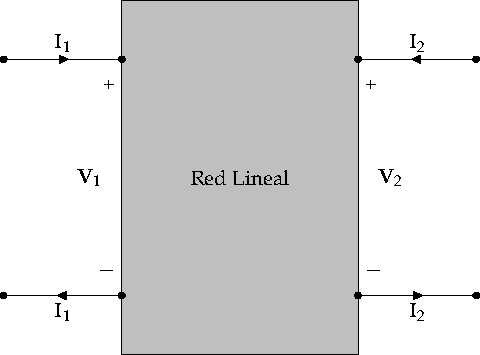
\includegraphics[height=5cm]{../figs/cuadripolo.pdf}
  \caption{Cuadripolo genérico.}
  \label{fig:cuadripolo}
\end{figure}

Las relaciones pueden expresarse de forma diversa, dando lugar a diferentes familias de parámetros. En este capítulo distinguiremos cuatro familias:
\begin{itemize}
\item Parámetros impedancia: las tensiones se expresan en función de las corrientes.
\item Parámetros admitancia: las corrientes se expresan en función de las tensiones.
\item Parámetros híbridos: la tensión de entrada y la corriente de salida se expresan en función de la tensión de salida y la corriente de entrada.
\item Parámetros híbridos inversos: la corriente de entrada y la tensión de salida se expresan en función de la tensión de entrada y la corriente de salida.
\item Parámetros de transmisión: la tensión y la corriente de entrada se expresan en función de la tensión y la corriente de salida.
\item Parámetros de transmisión inversa: la tensión y la corriente de salida se expresan en función de la tensión y la corriente de entrada.
\end{itemize}

En estas relaciones es importante prestar atención al sentido de las corrientes. En las primeras cuatro familias las corrientes son entrantes al cuadripolo, pero en los parámetros de transmisión la corriente de salida es saliente.

En el resto del capítulo se supondrá que el circuito representado por el cuadripolo puede contener elementos pasivos (resistencias, bobinas, condensadores) y fuentes dependientes, pero no fuentes independientes.

Las ecuaciones que se recogen a continuación emplean una nomenclatura genérica válida tanto para Laplace como para fasores, empleando el resaltado en negrita para tensiones, corrientes e impedancias. Los parámetros del cuadripolo se muestran en minúsculas, y las impedancias del circuito en mayúsculas.

\subsubsection{Cuadripolos Recíprocos y Simétricos}

Un cuadripolo es recíproco si, al intercambiar la posición de las excitaciones, la respuesta en el puerto correspondiente no sufre cambios (teorema de reciprocidad). Un cuadripolo lineal sin fuentes dependientes es recíproco. Además, un cuadripolo recíproco es simétrico si se puede intercambiar la entrada con la salida (simetría física).

\section{Parámetros de Cuadripolos}

\subsection{Parámetros de Impedancia}
\label{sec:impedancia}

El circuito de la figura \ref{fig:cuadripolo-impedancia} representa un cuadripolo alimentado por fuentes de corriente tanto en la entrada como en la salida. Empleando el teorema de superposición podemos calcular las tensiones en los puertos de entrada y salida, teniendo en cuenta que las variables independientes (los \emph{generadores}) son \(\mathbf{I}_1\) e \(\mathbf{I}_2\). Obtenemos las ecuaciones \ref{eq:parametros-impedancia}, en las que aparecen los parámetros impedancia $\mathbf{z}_{ij}$ relacionando las tensiones con las corrientes: 

\begin{figure}[H]
  \centering
  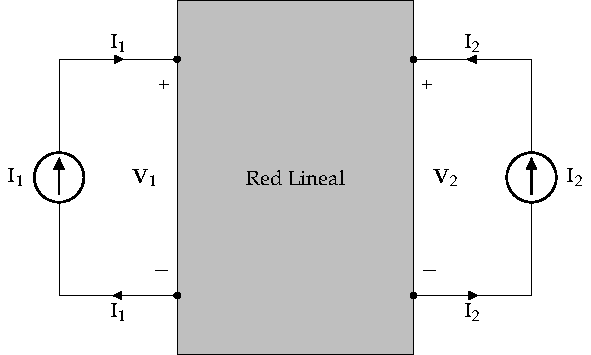
\includegraphics[height=4cm]{../figs/cuadripolo_fuentes_corriente.pdf}
  \caption{Cuadripolo alimentado por sendas fuentes de corriente.}
  \label{fig:cuadripolo-impedancia}
\end{figure}


\begin{equation}
  \label{eq:parametros-impedancia}
  \begin{array}{l}
    \mathbf{U}_1 = \mathbf{z}_{11} \mathbf{I}_1 + \mathbf{z}_{12} \mathbf{I}_2\\
    \mathbf{U}_2 = \mathbf{z}_{21} \mathbf{I}_1 + \mathbf{z}_{22} \mathbf{I}_2\\
  \end{array}
\end{equation}

La expresión matricial correspondiente, ecuación \ref{eq:parametros-impedancia-matriz}, contiene la matriz de parámetros impedancia:

\begin{equation}
  \label{eq:parametros-impedancia-matriz}
  \left[
    \begin{array}{c}
      \mathbf{U}_1\\
      \mathbf{U}_2
    \end{array}
  \right] =
  \left[
    \begin{array}{cc}
      \mathbf{z}_{11} & \mathbf{z}_{12}\\
      \mathbf{z}_{21} & \mathbf{z}_{22}
    \end{array}
  \right] \cdot
  \left[
    \begin{array}{c}
      \mathbf{I}_1\\
      \mathbf{I}_2
    \end{array}
  \right]
\end{equation}

Estas ecuaciones pueden representarse mediante un circuito equivalente, figura \ref{fig:circuito-equivalente-impedancia}, que contiene una impedancia de entrada, una impedancia de salida, y sendas fuentes de tensión dependientes.
\begin{figure}[H]
  \centering
  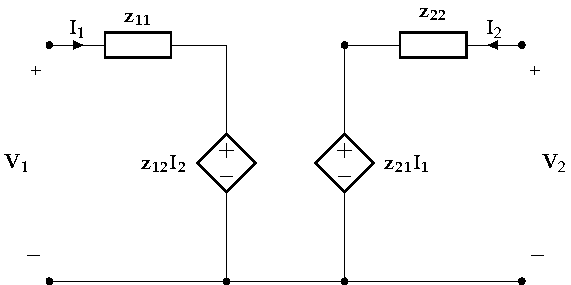
\includegraphics[height=4cm]{../figs/circuitoEquivalenteZ.pdf}
  \caption{Circuito equivalente de un cuadripolo caracterizado por parámetros impedancia.}
  \label{fig:circuito-equivalente-impedancia}
\end{figure}

\subsubsection{Cálculo de parámetros}

Para el cálculo de los parámetros recurrimos al teorema de superposición, activando y apagando las fuentes adecuadas para la obtención del parámetro deseado.

En primer lugar, con la salida del cuadripolo en abierto (figura \ref{fig:medida-impedancia-entrada}), es decir, apagando la fuente de corriente $I_2$, se obtienen los parámetros $\mathbf{z_{11}}$ y $\mathbf{z_{21}}$:
\[
  \begin{array}{c}
    \mathbf{z}_{11} = \left.\frac{\mathbf{U}_1}{\mathbf{I}_1}\right\rvert_{\mathbf{I}_2 = 0} \\
    \mathbf{z}_{21} = \left.\frac{\mathbf{U}_2}{\mathbf{I}_1}\right\rvert_{\mathbf{I}_2 = 0}
  \end{array}
\]

\begin{figure}[H]
  \centering
  \subfloat[$\mathbf{z}_{11}$ y $\mathbf{z}_{21}$]{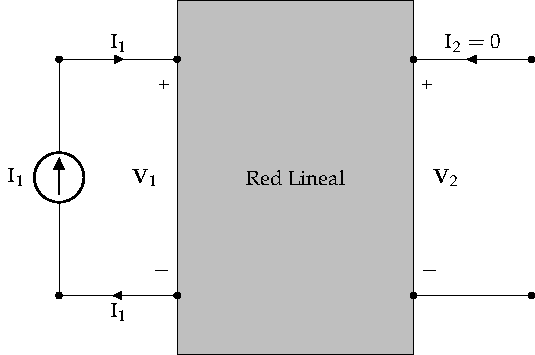
\includegraphics[height=4cm]{../figs/parametrosZ_entrada.pdf}\label{fig:medida-impedancia-entrada}}\hspace{2cm}
  \subfloat[$\mathbf{z}_{12}$ y $\mathbf{z}_{22}$]{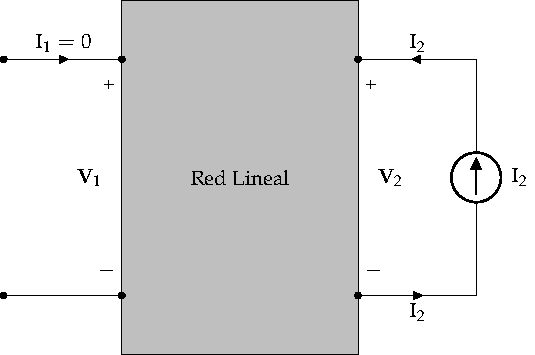
\includegraphics[height=4cm]{../figs/parametrosZ_salida.pdf}\label{fig:medida-impedancia-salida}}
\caption{Circuitos de medida para la obtención de los parámetros impedancia.}
  \label{fig:medida-impedancia}
\end{figure}


A continuación, con la entrada en abierto (figura \ref{fig:medida-impedancia-salida}), se obtienen los parámetros $\mathbf{z}_{22}$ y $\mathbf{z}_{12}$:

\[
  \begin{array}{c}
    \mathbf{z}_{12} = \left.\frac{\mathbf{U}_1}{\mathbf{I}_2}\right\rvert_{\mathbf{I}_1 = 0}\\
    \mathbf{z}_{22} = \left.\frac{\mathbf{U}_2}{\mathbf{I}_2}\right\rvert_{\mathbf{I}_1 = 0}
  \end{array}
\]


\subsubsection{Reciprocidad}

En el caso de un cuadripolo recíproco, al intercambiar la posición de una fuente de corriente manteniendo el otro puerto en circuito abierto (figura \ref{fig:impedancia-reciprocidad}), la tensión en circuito abierto será la misma:

\[
\left.\mathbf{U_1}\right\rvert_{
  \begin{array}{l}
\mathbf{I_1} = 0\\ \mathbf{I_2} = \mathbf{I_x}
  \end{array}
} =% 
\left.\mathbf{U_2}\right\rvert_{
  \begin{array}{l}
\mathbf{I_2} = 0\\ \mathbf{I_1} = \mathbf{I_x}
  \end{array}
} = \mathbf{U}_x
\]

\begin{figure}[H]
  \centering
  \subfloat[Fuente en la salida]{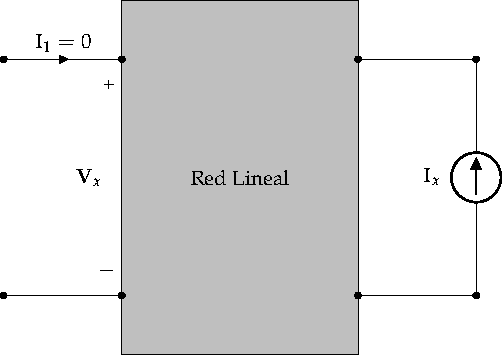
\includegraphics[height=4cm]{../figs/reciprocidadZ_entrada.pdf}}\hspace{2cm}
  \subfloat[Fuente en la entrada]{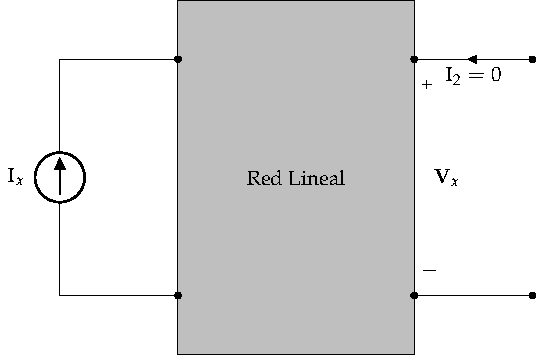
\includegraphics[height=4cm]{../figs/reciprocidadZ_salida.pdf}}
  \caption{Cuadripolo recíproco alimentado por fuentes de corriente.}
  \label{fig:impedancia-reciprocidad}
\end{figure}


Empleando esta relación con los parámetros impedancia, se comprueba que las impedancias de transferencia $\mathbf{z}_{12}$ y $\mathbf{z}_{21}$ son idénticas:
\[
  \left.
    \begin{array}{l}
      \mathbf{U}_x = \mathbf{z}_{11} 0  + \mathbf{z}_{12} \mathbf{I}_x\\
      \mathbf{U}_x = \mathbf{z}_{21} \mathbf{I}_x + \mathbf{z}_{22} 0\\
    \end{array} \right\} \rightarrow \mathbf{z_{12}} = \mathbf{z_{21}}
\]
de forma que la matriz de impedancias es simétrica:
\[
\left[
    \begin{array}{c}
      \mathbf{U}_1\\
      \mathbf{U}_2
    \end{array}
  \right] =
  \left[
    \begin{array}{cc}
      \mathbf{z}_{11} & \color{red}{\mathbf{z}_{12}}\\
      \color{red}{\mathbf{z}_{12}} & \mathbf{z}_{22}
    \end{array}
  \right] \cdot
  \left[
    \begin{array}{c}
      \mathbf{I}_1\\
      \mathbf{I}_2
    \end{array}
  \right]
\]

Con este resultado se puede demostrar fácilmente que un cuadripolo recíproco es equivalente al circuito en T de la figura \ref{fig:impedancia-equivalente-recíproco}:

\begin{figure}[H]
  \centering
  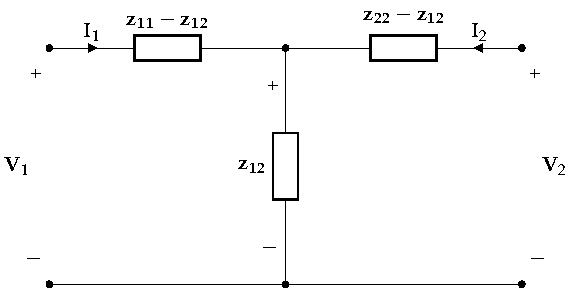
\includegraphics[height=4cm]{../figs/circuitoEquivalenteZReciproco.pdf}
  \caption{Circuito en T equivalente de un cuadripolo recíproco.}
  \label{fig:impedancia-equivalente-recíproco}
\end{figure}

En este circuito, si el cuadripolo es simétrico, las impedancias de entrada y salida deben ser idénticas (figura \ref{fig:impedancia-equivalente-simétrico}). Por tanto, en un cuadripolo simétrico $\mathbf{z_{11}} = \mathbf{z_{22}}$.
\begin{figure}[H]
  \centering
  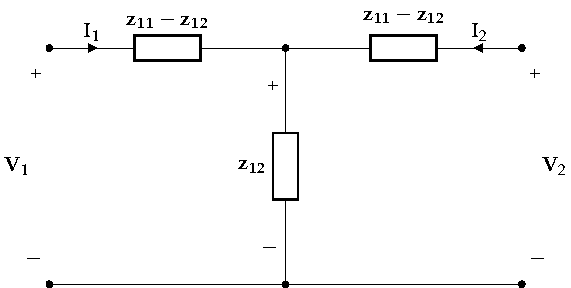
\includegraphics[height=4cm]{../figs/circuitoEquivalenteZSimetrico.pdf}
  \caption{Circuito en T equivalente de un cuadripolo simétrico.}
  \label{fig:impedancia-equivalente-simétrico}
\end{figure}

\[
  \left[
    \begin{array}{c}
      \mathbf{U}_1\\
      \mathbf{U}_2
    \end{array}
  \right] =
  \left[
    \begin{array}{cc}
      \color{blue}{\mathbf{z}_{11}} & \color{red}{\mathbf{z}_{12}}\\
      \color{red}{\mathbf{z}_{12}} & \color{blue}{\mathbf{z}_{11}}
    \end{array}
  \right] \cdot
  \left[
    \begin{array}{c}
      \mathbf{I}_1\\
      \mathbf{I}_2
    \end{array}
  \right]
\]

En resumen, un cuadripolo queda caracterizado por cuatro parámetros impedancia, siendo necesarios tres en el caso de un cuadripolo recíproco, y únicamente dos si el cuadripolo es simétrico.

Cerraremos esta sección haciendo notar que no todos los circuitos pueden ser modelados mediante un cuadripolo con parámetros impedancia. Queda como propuesta para el lector interesado comprobar esta circunstancia con un transformador ideal o con una impedancia en serie entre la entrada y la salida.

\subsection{Parámetros de Admitancia}

El circuito de la figura \ref{fig:cuadripolo-admitancia} representa un cuadripolo alimentado por fuentes de tensión tanto en la entrada como en la salida. Empleando el teorema de superposición podemos calcular las corrientes en los puertos de entrada y salida, teniendo en cuenta que las variables independientes (los \emph{generadores}) son \(\mathbf{U}_1\) e \(\mathbf{U}_2\). En este caso, obtenemos las ecuaciones \ref{eq:parametros-admitancia}, en las que aparecen los parámetros admitancia $\mathbf{y}_{ij}$ relacionando las corrientes con las tensiones: 

\begin{figure}[H]
  \centering
  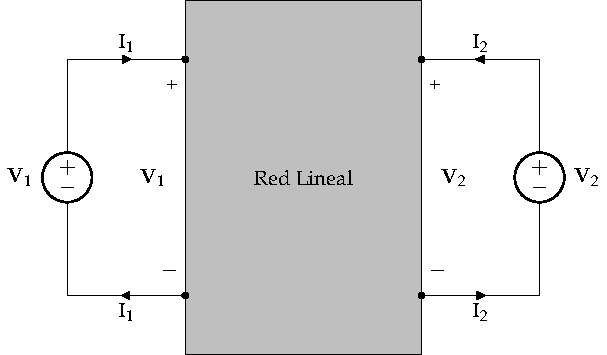
\includegraphics[height=4cm]{../figs/cuadripolo_fuentes_tension.pdf}
  \caption{Cuadripolo alimentado por sendas fuentes de tensión.}
  \label{fig:cuadripolo-admitancia}
\end{figure}


\begin{equation}
  \label{eq:parametros-admitancia}
  \begin{array}{l}
  \mathbf{I}_1 = \mathbf{y}_{11} \mathbf{U}_1 + \mathbf{y}_{12} \mathbf{U}_2\\
  \mathbf{I}_2 = \mathbf{y}_{21} \mathbf{U}_1 + \mathbf{y}_{22} \mathbf{U}_2\\
  \end{array}
\end{equation}

La expresión matricial correspondiente, ecuación \ref{eq:parametros-admitancia-matriz}, contiene la matriz de parámetros admitancia:


\begin{equation}
  \label{eq:parametros-admitancia-matriz}
  \left[
    \begin{array}{c}
      \mathbf{I}_1\\
      \mathbf{I}_2
    \end{array}
  \right] =
  \left[
    \begin{array}{cc}
      \mathbf{y}_{11} & \mathbf{y}_{12}\\
      \mathbf{y}_{21} & \mathbf{y}_{22}
    \end{array}
  \right] \cdot
  \left[
    \begin{array}{c}
      \mathbf{U}_1\\
      \mathbf{U}_2
    \end{array}
  \right]
\end{equation}

Estas ecuaciones pueden representarse mediante un circuito equivalente, figura \ref{fig:circuito-equivalente-admitancia}, que contiene una admitancia de entrada, una admitancia de salida, y sendas fuentes de corriente dependientes.

\begin{figure}[H]
  \centering
  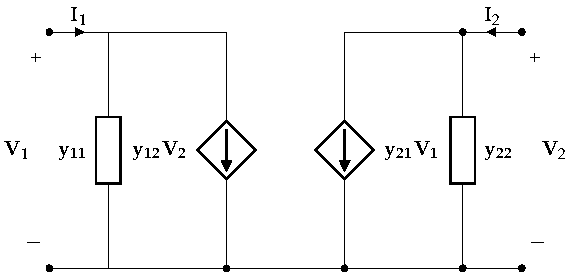
\includegraphics[height=4cm]{../figs/circuitoEquivalenteY.pdf}
  \caption{Circuito equivalente de un cuadripolo caracterizado por parámetros impedancia.}
  \label{fig:circuito-equivalente-admitancia}
\end{figure}


\subsubsection{Cálculo de parámetros}

Para el cálculo de los parámetros recurrimos al teorema de superposición, activando y apagando las fuentes adecuadas para la obtención del parámetro deseado.

En primer lugar, con la salida del cuadripolo en cortocircuito (figura \ref{fig:medida-admitancia-entrada}), es decir, apagando la fuente de tensión $U_2$, se obtienen los parámetros $\mathbf{y_{11}}$ y $\mathbf{y_{21}}$:

\[
  \begin{array}{c}
    \mathbf{y}_{11} = \left.\frac{\mathbf{I}_1}{\mathbf{U}_1}\right\rvert_{\mathbf{U}_2 = 0} \\
    \mathbf{y}_{21} = \left.\frac{\mathbf{I}_2}{\mathbf{U}_1}\right\rvert_{\mathbf{U}_2 = 0}
  \end{array}
\]

\begin{figure}[H]
  \centering
  \subfloat[$\mathbf{y}_{11}$ e $\mathbf{y}_{21}$]{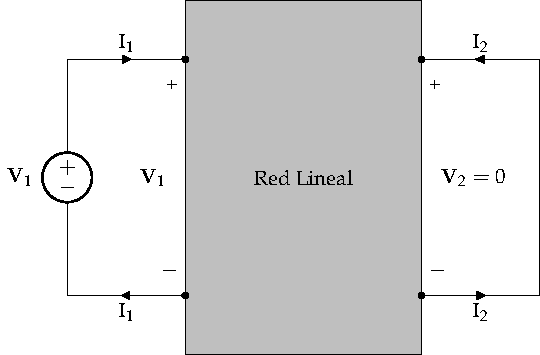
\includegraphics[height=4cm]{../figs/parametrosY_entrada.pdf}\label{fig:medida-admitancia-entrada}}\hspace{2cm}
  \subfloat[$\mathbf{y}_{12}$ e $\mathbf{y}_{22}$]{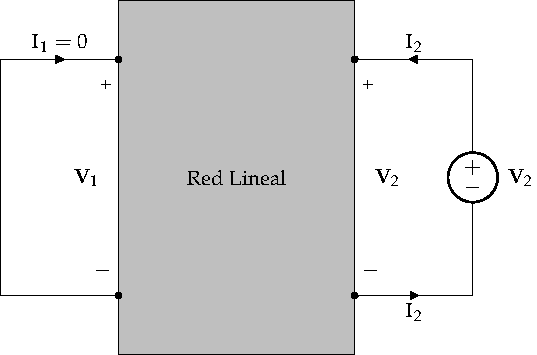
\includegraphics[height=4cm]{../figs/parametrosY_salida.pdf}\label{fig:medida-admitancia-salida}}
\caption{Circuitos de medida para la obtención de los parámetros admitancia.}
  \label{fig:medida-admitancia}
\end{figure}

A continuación, con la entrada en cortocircuito (figura \ref{fig:medida-admitancia-salida}), se obtienen los parámetros $\mathbf{y}_{22}$ y $\mathbf{y}_{12}$:

\[
  \begin{array}{c}
    \mathbf{y}_{12} = \left.\frac{\mathbf{I}_1}{\mathbf{U}_2}\right\rvert_{\mathbf{U}_1 = 0}\\
    \mathbf{y}_{22} = \left.\frac{\mathbf{I}_2}{\mathbf{U}_2}\right\rvert_{\mathbf{U}_1 = 0}
  \end{array}
\]


\subsubsection{Reciprocidad}

En el caso de un cuadripolo recíproco, al intercambiar la posición de
una fuente de tensión manteniendo el otro puerto en cortocircuito
(figura \ref{fig:admitancia-reciprocidad}), la corriente de
cortocircuito será la misma:

\[
  \mathbf{I_1}\rvert_{
    \begin{array}{l}
      \mathbf{U_1} = 0 \\ \mathbf{U_2} = \mathbf{U_x}
    \end{array}
  } =%
  \mathbf{I_2}\rvert_{
    \begin{array}{l}
      \mathbf{U_2} = 0 \\ \mathbf{U_1} = \mathbf{U_x}
    \end{array}
  }
\]

\begin{figure}[H]
  \centering \subfloat[Fuente en la
  salida]{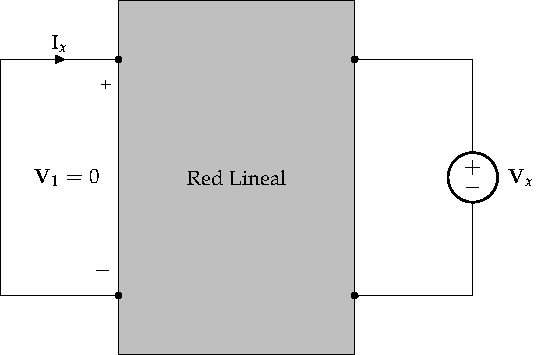
\includegraphics[height=4cm]{../figs/reciprocidadY_entrada.pdf}}\hspace{2cm}
  \subfloat[Fuente en la
  entrada]{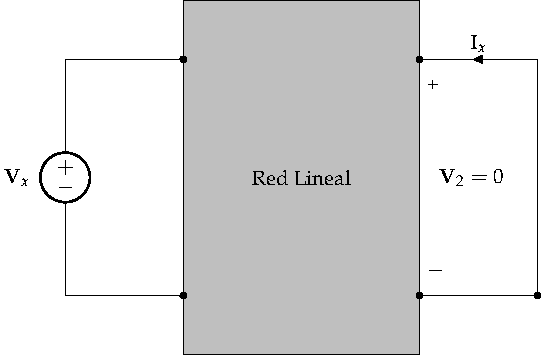
\includegraphics[height=4cm]{../figs/reciprocidadY_salida.pdf}}
  \caption{Cuadripolo recíproco alimentado por fuentes de tensión.}
  \label{fig:admitancia-reciprocidad}
\end{figure}

Empleando esta relación con los parámetros admitancia, se comprueba
que las admitancia de transferencia $\mathbf{y}_{12}$ e
$\mathbf{y}_{21}$ son idénticas:
\[
  \left.
    \begin{array}{l}
      \mathbf{I}_x = \mathbf{y}_{11} 0  + \mathbf{y}_{12} \mathbf{U}_x\\
      \mathbf{I}_x = \mathbf{y}_{21} \mathbf{U}_x + \mathbf{y}_{22} 0\\
    \end{array} \right\} \rightarrow \mathbf{y_{12}} = \mathbf{y_{21}}
\]
de forma que la matriz de admitancias es simétrica:
\[
  \left[
    \begin{array}{c}
      \mathbf{I}_1\\
      \mathbf{I}_2
    \end{array}
  \right] = \left[
    \begin{array}{cc}
      \mathbf{y}_{11} & \color{red}{\mathbf{y}_{12}}\\
      \color{red}{\mathbf{y}_{12}} & \mathbf{y}_{22}
    \end{array}
  \right] \cdot \left[
    \begin{array}{c}
      \mathbf{U}_1\\
      \mathbf{U}_2
    \end{array}
  \right]
\]

Con este resultado se puede demostrar fácilmente que un cuadripolo
recíproco es equivalente al circuito en $\pi$ de la figura
\ref{fig:admitancia-equivalente-recíproco}:

\begin{figure}[H]
  \centering
  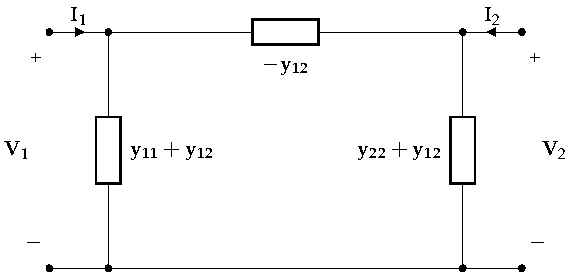
\includegraphics[height=4cm]{../figs/circuitoEquivalenteYReciproco.pdf}
  \caption{Circuito en $\pi$ equivalente de un cuadripolo recíproco.}
  \label{fig:admitancia-equivalente-recíproco}
\end{figure}

En este circuito, si el cuadripolo es simétrico, las admitancias de
entrada y salida deben ser idénticas (figura
\ref{fig:admitancia-equivalente-simétrico}). Por tanto, en un
cuadripolo simétrico $\mathbf{y_{11}} = \mathbf{y_{22}}$.
\begin{figure}[H]
  \centering
  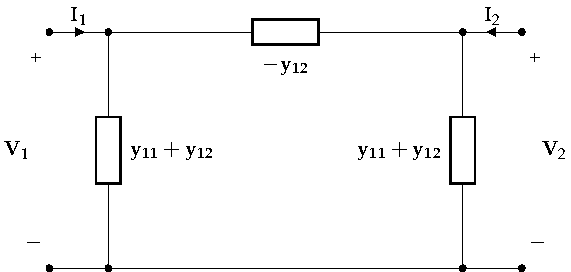
\includegraphics[height=4cm]{../figs/circuitoEquivalenteYSimetrico.pdf}
  \caption{Circuito en $\pi$ equivalente de un cuadripolo simétrico.}
  \label{fig:admitancia-equivalente-simétrico}
\end{figure}


\[
  \left[
    \begin{array}{c}
      \mathbf{I}_1\\
      \mathbf{I}_2
    \end{array}
  \right] = \left[
    \begin{array}{cc}
      \color{blue}{\mathbf{y}_{11}} & \color{red}{\mathbf{y}_{12}}\\
      \color{red}{\mathbf{y}_{12}} & \color{blue}{\mathbf{y}_{11}}
    \end{array}
  \right] \cdot \left[
    \begin{array}{c}
      \mathbf{U}_1\\
      \mathbf{U}_2
    \end{array}
  \right]
\]

En resumen, un cuadripolo queda caracterizado por cuatro parámetros
admitancia, siendo necesarios tres en el caso de un cuadripolo
recíproco, y únicamente dos si el cuadripolo es simétrico.

De la misma forma que con los parámetros admitancia, cerraremos la
sección haciendo notar que no todos los circuitos pueden ser modelados
mediante un cuadripolo con parámetros admitancia, como puede
comprobarse con un transformador ideal o una impedancia en paralelo
entre la entrada y la salida.


\subsection{Parámetros Híbridos}

El circuito de la figura \ref{fig:cuadripolo-hibridos} representa un
cuadripolo alimentado por una fuente de corriente en la entrada y una
fuente de tensión en la salida. En este montaje se pueden obtener la
tensión en la entrada y la corriente en la salida a partir de las
variables independientes \(\mathbf{I}_1\) y \(\mathbf{U}_2\). En este
caso, obtenemos las ecuaciones \ref{eq:parametros-hibridos}, en las
que aparecen los parámetros híbridos $\mathbf{h}_{ij}$:

\begin{figure}[H]
  \centering
  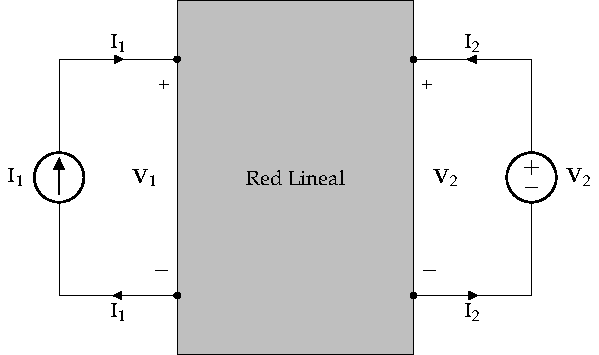
\includegraphics[height=4cm]{../figs/cuadripolo_hibrido.pdf}
  \caption{Cuadripolo alimentado por una fuente de corriente en la
    entrada y una fuente de tensión en la salida.}
  \label{fig:cuadripolo-hibridos}
\end{figure}



\begin{equation}
  \label{eq:parametros-hibridos}
  \begin{array}{l}
    \mathbf{U}_1 = \mathbf{h}_{11} \mathbf{I}_1 + \mathbf{h}_{12} \mathbf{U}_2\\
    \mathbf{I}_2 = \mathbf{h}_{21} \mathbf{I}_1 + \mathbf{h}_{22} \mathbf{U}_2\\
  \end{array}
\end{equation}

La expresión matricial correspondiente, ecuación \ref{eq:parametros-hibridos-matriz}, contiene la matriz de parámetros híbridos:

\begin{equation}
  \label{eq:parametros-hibridos-matriz}
  \left[
    \begin{array}{c}
      \mathbf{U}_1\\
      \mathbf{I}_2
    \end{array}
  \right] = \left[
    \begin{array}{cc}
      \mathbf{h}_{11} & \mathbf{h}_{12}\\
      \mathbf{h}_{21} & \mathbf{h}_{22}
    \end{array}
  \right] \cdot \left[
    \begin{array}{c}
      \mathbf{I}_1\\
      \mathbf{U}_2
    \end{array}
  \right]
\end{equation}

El circuito asociado a estas ecuaciones se representa en la figura \ref{fig:circuito-equivalente-hibridos}, que contiene una impedancia de entrada en serie con una fuente de tensión dependiente, y una admitancia de salida en paralelo con una fuente de corriente dependiente.

\begin{figure}[H]
  \centering
  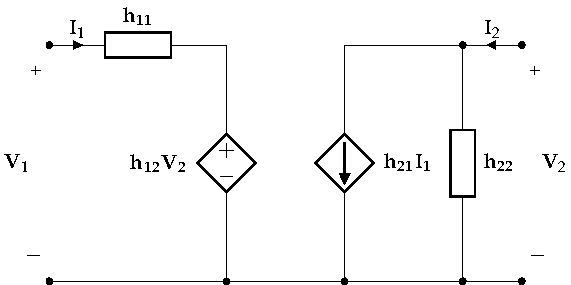
\includegraphics[height=4cm]{../figs/circuitoEquivalenteH.pdf}
  \caption{Circuito equivalente de un cuadripolo caracterizado por parámetros híbridos.}
  \label{fig:circuito-equivalente-hibridos}
\end{figure}


\subsubsection{Cálculo de parámetros}

Para el cálculo de los parámetros nuevamente recurrimos al teorema de superposición, activando y apagando las fuentes adecuadas para la obtención del parámetro deseado.

En primer lugar, con la salida del cuadripolo en cortocircuito (figura \ref{fig:medida-hibridos-entrada}), es decir, apagando la fuente de tensión $U_2$, se obtienen los parámetros $\mathbf{h_{11}}$ y $\mathbf{h_{21}}$:
    \[
      \begin{array}{c}
        \mathbf{h}_{11} = \left.\frac{\mathbf{U}_1}{\mathbf{I}_1}\right\rvert_{\mathbf{U}_2 = 0} \\
        \mathbf{h}_{21} = \left.\frac{\mathbf{I}_2}{\mathbf{I}_1}\right\rvert_{\mathbf{U}_2 = 0}
      \end{array}
    \]

\begin{figure}[H]
  \centering
  \subfloat[$\mathbf{h}_{11}$ y $\mathbf{h}_{21}$]{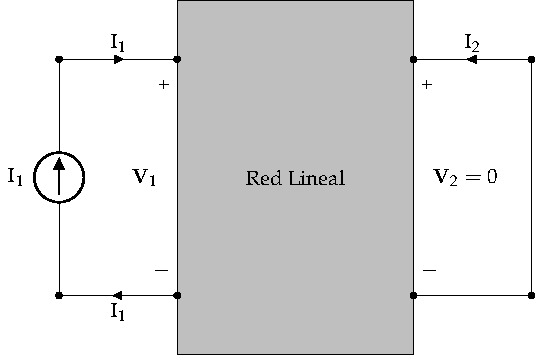
\includegraphics[height=4cm]{../figs/parametrosH_entrada.pdf}\label{fig:medida-hibridos-entrada}}\hspace{2cm}
  \subfloat[$\mathbf{h}_{12}$ y $\mathbf{h}_{22}$]{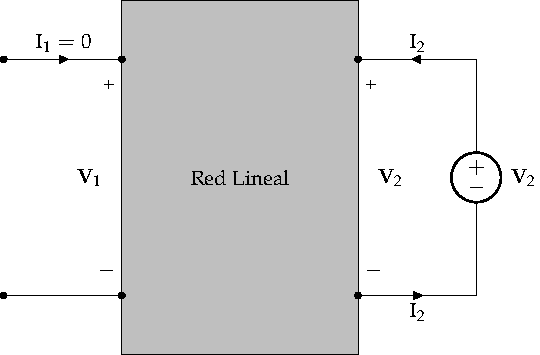
\includegraphics[height=4cm]{../figs/parametrosH_salida.pdf}\label{fig:medida-hibridos-salida}}
\caption{Circuitos de medida para la obtención de los parámetros híbridos.}
  \label{fig:medida-hibridos}
\end{figure}


A continuación, con la entrada en circuito abierto (figura \ref{fig:medida-hibridos-salida}), se obtienen los parámetros $\mathbf{h}_{22}$ y $\mathbf{h}_{12}$:

\[
  \begin{array}{c}
    \mathbf{h}_{12} = \left.\frac{\mathbf{U}_1}{\mathbf{U}_2}\right\rvert_{\mathbf{I}_1 = 0}\\
    \mathbf{h}_{22} = \left.\frac{\mathbf{I}_2}{\mathbf{U}_2}\right\rvert_{\mathbf{I}_1 = 0}
  \end{array}
\]


\subsection{Parámetros Híbridos Inversos}

El circuito de la figura \ref{fig:cuadripolo-hibridos-inversos}
representa un cuadripolo alimentado por una fuente de tensión en la
entrada y una fuente de corriente en la salida. En este montaje se
pueden obtener la corriente en la entrada y la tensión en la salida a
partir de las variables independientes \(\mathbf{U}_1\) e
\(\mathbf{I}_2\). En este caso, obtenemos las ecuaciones
\ref{eq:parametros-hibridos-inversos}, en las que aparecen los
parámetros híbridos inversos $\mathbf{g}_{ij}$:

\begin{figure}[H]
  \centering
  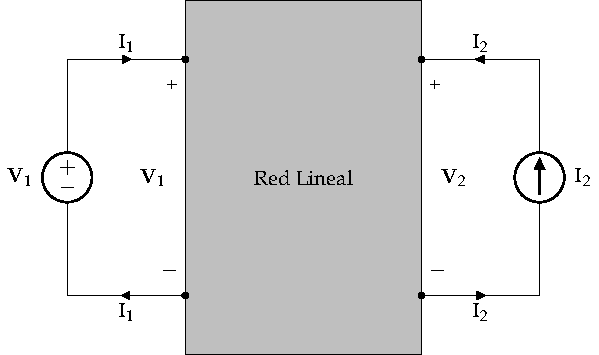
\includegraphics[height=4cm]{../figs/cuadripolo_hibrido_inverso.pdf}
  \caption{Cuadripolo alimentado por una fuente de tensión en la
    entrada y una fuente de corriente en la salida.}
  \label{fig:cuadripolo-hibridos-inversos}
\end{figure}

\begin{equation}
  \label{eq:parametros-hibridos-inversos}
    \begin{array}{l}
      \mathbf{I}_1 = \mathbf{g}_{11} \mathbf{U}_1 + \mathbf{g}_{12} \mathbf{I}_2\\
      \mathbf{U}_2 = \mathbf{g}_{21} \mathbf{U}_1 + \mathbf{g}_{22} \mathbf{I}_2\\
    \end{array}
\end{equation}

La expresión matricial correspondiente, ecuación
\ref{eq:parametros-hibridos-inversos-matriz}, contiene la matriz de
parámetros híbridos inversos:

\begin{equation}
  \label{eq:parametros-hibridos-inversos-matriz}
  \left[
    \begin{array}{c}
      \mathbf{I}_1\\
      \mathbf{U}_2
    \end{array}
  \right] =
  \left[
    \begin{array}{cc}
      \mathbf{g}_{11} & \mathbf{g}_{12}\\
      \mathbf{g}_{21} & \mathbf{g}_{22}
    \end{array}
  \right] \cdot
  \left[
    \begin{array}{c}
      \mathbf{U}_1\\
      \mathbf{I}_2
    \end{array}
  \right]
\end{equation}

El circuito asociado a estas ecuaciones se representa en la figura \ref{fig:circuito-equivalente-hibridos-inversos}, que contiene una admitancia de entrada en paralelo con una fuente de corriente dependiente, y una impedancia de salida en serie con una fuente de tensión dependiente.

\begin{figure}[H]
  \centering
  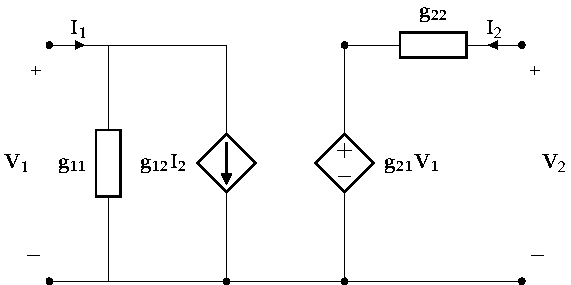
\includegraphics[height=4cm]{../figs/circuitoEquivalenteG.pdf}
  \caption{Circuito equivalente de un cuadripolo caracterizado por parámetros híbridos inversos.}
  \label{fig:circuito-equivalente-hibridos-inversos}
\end{figure}


\subsubsection{Cálculo de parámetros}

Para el cálculo de los parámetros nuevamente recurrimos al teorema de superposición, activando y apagando las fuentes adecuadas para la obtención del parámetro deseado.

En primer lugar, con la salida del cuadripolo en circuito abierto (figura \ref{fig:medida-hibridos-inversos-entrada}), es decir, apagando la fuente de corriente $I_2$, se obtienen los parámetros $\mathbf{g_{11}}$ y $\mathbf{g_{21}}$:
\[
  \begin{array}{c}
    \mathbf{g}_{11} = \left.\frac{\mathbf{I}_1}{\mathbf{U}_1}\right\rvert_{\mathbf{I}_2 = 0} \\
    \mathbf{g}_{21} = \left.\frac{\mathbf{U}_2}{\mathbf{U}_1}\right\rvert_{\mathbf{I}_2 = 0}
  \end{array}
\]
    
\begin{figure}[H]
  \centering
  \subfloat[$\mathbf{g}_{11}$ y $\mathbf{g}_{21}$]{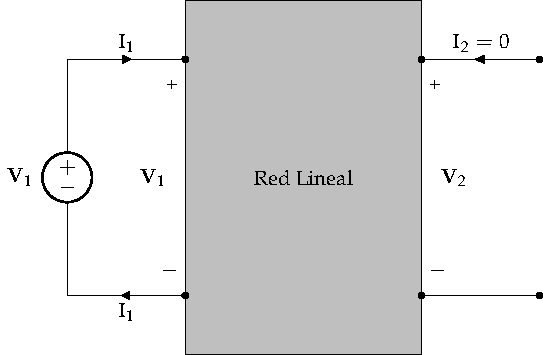
\includegraphics[height=4cm]{../figs/parametrosG_entrada.pdf}\label{fig:medida-hibridos-inversos-entrada}}\hspace{2cm}
  \subfloat[$\mathbf{g}_{12}$ y $\mathbf{g}_{22}$]{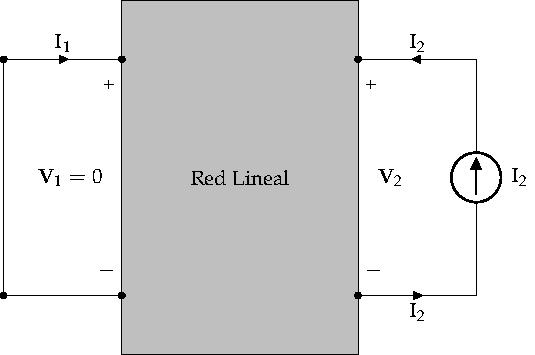
\includegraphics[height=4cm]{../figs/parametrosG_salida.pdf}\label{fig:medida-hibridos-inversos-salida}}
\caption{Circuitos de medida para la obtención de los parámetros híbridos inversos.}
  \label{fig:medida-hibridos-inversos}
\end{figure}


A continuación, con la entrada en cortocircuito (figura \ref{fig:medida-hibridos-inversos-salida}), se obtienen los parámetros $\mathbf{g}_{22}$ y $\mathbf{g}_{12}$:
\[
  \begin{array}{c}
    \mathbf{g}_{12} = \left.\frac{\mathbf{I}_1}{\mathbf{I}_2}\right\rvert_{\mathbf{U}_1 = 0}\\
    \mathbf{g}_{22} = \left.\frac{\mathbf{U}_2}{\mathbf{I}_2}\right\rvert_{\mathbf{U}_1 = 0}
  \end{array}
\]


\subsection{Parámetros de Transmisión}
\label{sec:orgd5598b8}

\subsubsection{Definición}
\label{sec:orgcd755d3}

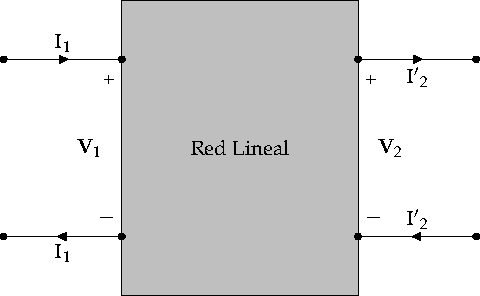
\includegraphics[height=4cm]{../figs/cuadripolo_transmision.pdf}


\[
\begin{array}{l}
  \mathbf{U}_1 = \mathbf{A} \mathbf{U}_2 + \mathbf{B}\mathbf{I'}_2\\
  \mathbf{I}_1 = \mathbf{C} \mathbf{U}_2 + \mathbf{D} \mathbf{I'}_2\\
\end{array}
\]


\textbf{Atención} al sentido de la corriente \(\mathbf{I'}_2\). (\(\mathbf{I'}_2 = - \mathbf{I}_2\)).


\subsubsection{Expresión Matricial}
\label{sec:org104daf9}

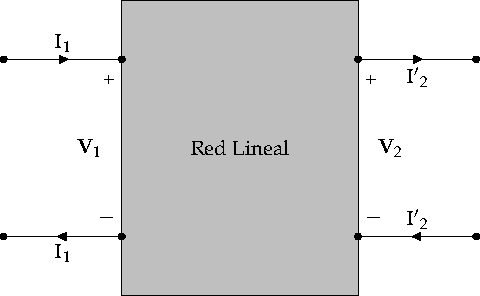
\includegraphics[height=4cm]{../figs/cuadripolo_transmision.pdf}


\[
  \left[
    \begin{array}{c}
      \mathbf{U}_1\\
      \mathbf{I}_1
    \end{array}
  \right] =
  \left[
    \begin{array}{cc}
      \mathbf{A} & \mathbf{B}\\
      \mathbf{C} & \mathbf{D}
    \end{array}
  \right] \cdot
  \left[
    \begin{array}{c}
      \mathbf{U}_2\\
      \mathbf{I'}_2
    \end{array}
  \right]
\]

\subsubsection{Cálculo de parámetros}
\label{sec:org99ce061}

Se debe medir el inverso de cada parámetro, dado que la magnitud a medir y la excitación pertenecen al mismo puerto.

\renewcommand{\arraystretch}{3}
\[
  \begin{array}{cc}
    \frac{1}{\mathbf{A}} = \left.\frac{\mathbf{U}_2}{\mathbf{U}_1}\right\rvert_{\mathbf{I}_2 = 0} &
    \frac{1}{\mathbf{B}} = \left.\frac{\mathbf{I'}_2}{\mathbf{U}_1}\right\rvert_{\mathbf{U}_2 = 0}\\
    \frac{1}{\mathbf{C}} = \left.\frac{\mathbf{U}_2}{\mathbf{I}_1}\right\rvert_{\mathbf{I}_2 = 0} &
    \frac{1}{\mathbf{D}} = \left.\frac{\mathbf{I'}_2}{\mathbf{I}_1}\right\rvert_{\mathbf{U}_2 = 0}\\
  \end{array}
\]

\begin{enumerate}
\item \hfill{}\textsc{BMCOL}
\label{sec:orga42aeb3}

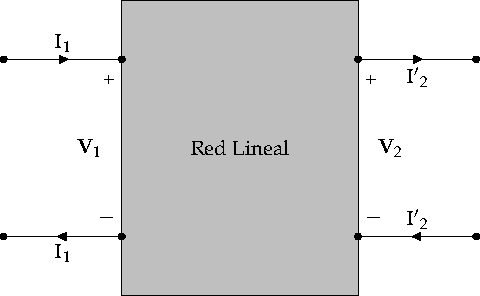
\includegraphics[height=4cm]{../figs/cuadripolo_transmision.pdf}


\item \hfill{}\textsc{BMCOL}
\label{sec:orgb82d084}
\renewcommand{\arraystretch}{1}
\[
\begin{array}{l}
  \mathbf{U}_1 = \mathbf{A} \mathbf{U}_2 + \mathbf{B}\mathbf{I'}_2\\
  \mathbf{I}_1 = \mathbf{C} \mathbf{U}_2 + \mathbf{D} \mathbf{I'}_2\\
\end{array}
\]
\end{enumerate}


\subsection{Parámetros de Transmisión Inversa}
\label{sec:orgd62a71b}

\subsubsection{Definición}
\label{sec:org52b179c}

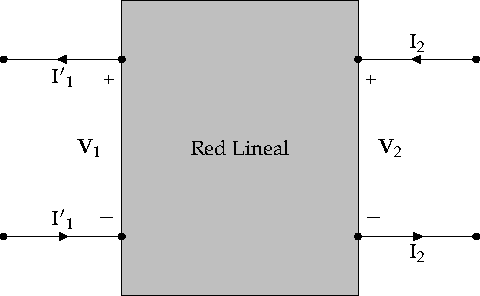
\includegraphics[height=4cm]{../figs/cuadripolo_transmision_inversa.pdf}


\[
\begin{array}{l}
  \mathbf{U}_2 = \mathbf{a} \mathbf{U}_1 + \mathbf{b}\mathbf{I'}_1\\
  \mathbf{I}_2 = \mathbf{c} \mathbf{U}_1 + \mathbf{d} \mathbf{I'}_1\\
\end{array}
\]


\textbf{Atención} al sentido de la corriente \(\mathbf{I'}_1\) (\(\mathbf{I'}_1 = - \mathbf{I}_1\)).


\subsubsection{Expresión Matricial}
\label{sec:orgca7fb03}

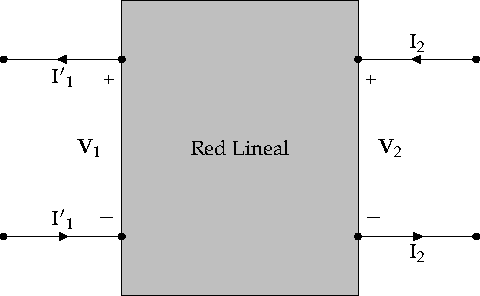
\includegraphics[height=4cm]{../figs/cuadripolo_transmision_inversa.pdf}


\[
  \left[
    \begin{array}{c}
      \mathbf{U}_2\\
      \mathbf{I}_2
    \end{array}
  \right] =
  \left[
    \begin{array}{cc}
      \mathbf{a} & \mathbf{b}\\
      \mathbf{c} & \mathbf{d}
    \end{array}
  \right] \cdot
  \left[
    \begin{array}{c}
      \mathbf{U}_1\\
      \mathbf{I'}_1
    \end{array}
  \right]
\]

\subsubsection{Cálculo de parámetros}
\label{sec:org67b01c0}
Se debe medir el inverso de cada parámetro, dado que la magnitud a medir y la excitación pertenecen al mismo puerto.

\renewcommand{\arraystretch}{3}
\[
  \begin{array}{cc}
    \frac{1}{\mathbf{a}} = \left.\frac{\mathbf{U}_1}{\mathbf{U}_2}\right\rvert_{\mathbf{I}_1 = 0} &
    \frac{1}{\mathbf{b}} = \left.\frac{\mathbf{I'}_1}{\mathbf{U}_2}\right\rvert_{\mathbf{U}_1 = 0}\\
    \frac{1}{\mathbf{c}} = \left.\frac{\mathbf{U}_1}{\mathbf{I}_2}\right\rvert_{\mathbf{I}_1 = 0} &
    \frac{1}{\mathbf{d}} = \left.\frac{\mathbf{I'}_1}{\mathbf{I}_2}\right\rvert_{\mathbf{U}_1 = 0}\\
  \end{array}
\]

\begin{enumerate}
\item \hfill{}\textsc{BMCOL}
\label{sec:org770263e}

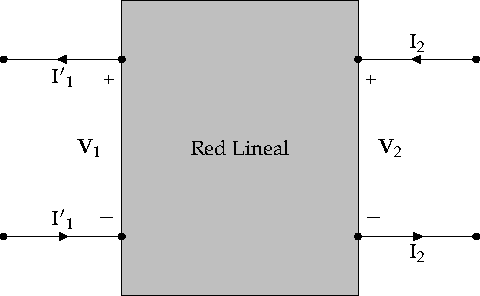
\includegraphics[height=4cm]{../figs/cuadripolo_transmision_inversa.pdf}


\item \hfill{}\textsc{BMCOL}
\label{sec:orgc57f0bc}
\renewcommand{\arraystretch}{1}
\[
\begin{array}{l}
  \mathbf{U}_2 = \mathbf{a} \mathbf{U}_1 + \mathbf{b}\mathbf{I'}_1\\
  \mathbf{I}_2 = \mathbf{c} \mathbf{U}_1 + \mathbf{d} \mathbf{I'}_1\\
\end{array}
\]
\end{enumerate}


\section{Relación entre parámetros}
\label{sec:org2eae33c}

\subsubsection{Impedancia y Admitancia}
\label{sec:orgf5948b7}
\[
  \left.
    \begin{array}{l}
      \left[
      \begin{array}{c}
        \mathbf{U}_1\\
        \mathbf{U}_2
      \end{array}
      \right] =
      \left[
      \begin{array}{cc}
        \mathbf{z}_{11} & \mathbf{z}_{12}\\
        \mathbf{z}_{21} & \mathbf{z}_{22}
      \end{array}
                          \right]
                          \cdot
                          \left[
                          \begin{array}{c}
                            \mathbf{I}_1\\
                            \mathbf{I}_2
                          \end{array}
      \right] \\ \\
      \left[
      \begin{array}{c}
        \mathbf{I}_1\\
        \mathbf{I}_2
      \end{array}
      \right] =
      \left[
      \begin{array}{cc}
        \mathbf{y}_{11} & \mathbf{y}_{12}\\
        \mathbf{y}_{21} & \mathbf{y}_{22}
      \end{array}
                          \right] \cdot
                          \left[
                          \begin{array}{c}
                            \mathbf{U}_1\\
                            \mathbf{U}_2
                          \end{array}
      \right]
    \end{array}
    \right\}
      \rightarrow
      \boxed{[\mathbf{Z}] = [\mathbf{Y}]^{-1}}
    \]

\subsubsection{Híbridos}
\label{sec:org34b878b}
\[
  \left.
    \begin{array}{l}
      %% Híbridos
  \left[
    \begin{array}{c}
      \mathbf{U}_1\\
      \mathbf{I}_2
    \end{array}
  \right] =
  \left[
    \begin{array}{cc}
      \mathbf{h}_{11} & \mathbf{h}_{12}\\
      \mathbf{h}_{21} & \mathbf{h}_{22}
    \end{array}
  \right] \cdot
  \left[
    \begin{array}{c}
      \mathbf{I}_1\\
      \mathbf{U}_2
    \end{array}
      \right]
      \\ \\
      %% Híbridos Inversos
  \left[
    \begin{array}{c}
      \mathbf{I}_1\\
      \mathbf{U}_2
    \end{array}
  \right] =
  \left[
    \begin{array}{cc}
      \mathbf{g}_{11} & \mathbf{g}_{12}\\
      \mathbf{g}_{21} & \mathbf{g}_{22}
    \end{array}
  \right] \cdot
  \left[
    \begin{array}{c}
      \mathbf{U}_1\\
      \mathbf{I}_2
    \end{array}
      \right]
      \end{array}
    \right\}
      \rightarrow
      \boxed{[\mathbf{H}] = [\mathbf{G}]^{-1}}
    \]
\subsubsection{Transmisión}
\label{sec:org47212d8}
\[
  \left.
    \begin{array}{l}
      %% Transmisión
  \left[
    \begin{array}{c}
      \mathbf{U}_1\\
      \mathbf{I}_1
    \end{array}
  \right] =
  \left[
    \begin{array}{cc}
      \mathbf{A} & \mathbf{B}\\
      \mathbf{C} & \mathbf{D}
    \end{array}
  \right] \cdot
  \left[
    \begin{array}{c}
      \mathbf{U}_2\\
      \mathbf{I'}_2
    \end{array}
  \right]
      \\ \\
      %% Transmisión Inversa
  \left[
    \begin{array}{c}
      \mathbf{U}_2\\
      \mathbf{I}_2
    \end{array}
  \right] =
  \left[
    \begin{array}{cc}
      \mathbf{a} & \mathbf{b}\\
      \mathbf{c} & \mathbf{d}
    \end{array}
  \right] \cdot
  \left[
    \begin{array}{c}
      \mathbf{U}_1\\
      \mathbf{I'}_1
    \end{array}
  \right]
      \end{array}
    \right\}
    \rightarrow
    \boxed{[\mathbf{T}] \neq [\mathbf{t}]^{-1}}
  \]
\[
  \boxed{
    \left[
      \begin{array}{cc}
        \mathbf{A} & \mathbf{B}\\
        \mathbf{C} & \mathbf{D}
      \end{array}\right] = 
      \left[
      \begin{array}{cc}
        \mathbf{a} & \mathbf{-b}\\
        \mathbf{-c} & \mathbf{d}
      \end{array}
      \right]^{-1}
    }
\]
\subsubsection{}
\label{sec:orgf3da70f}

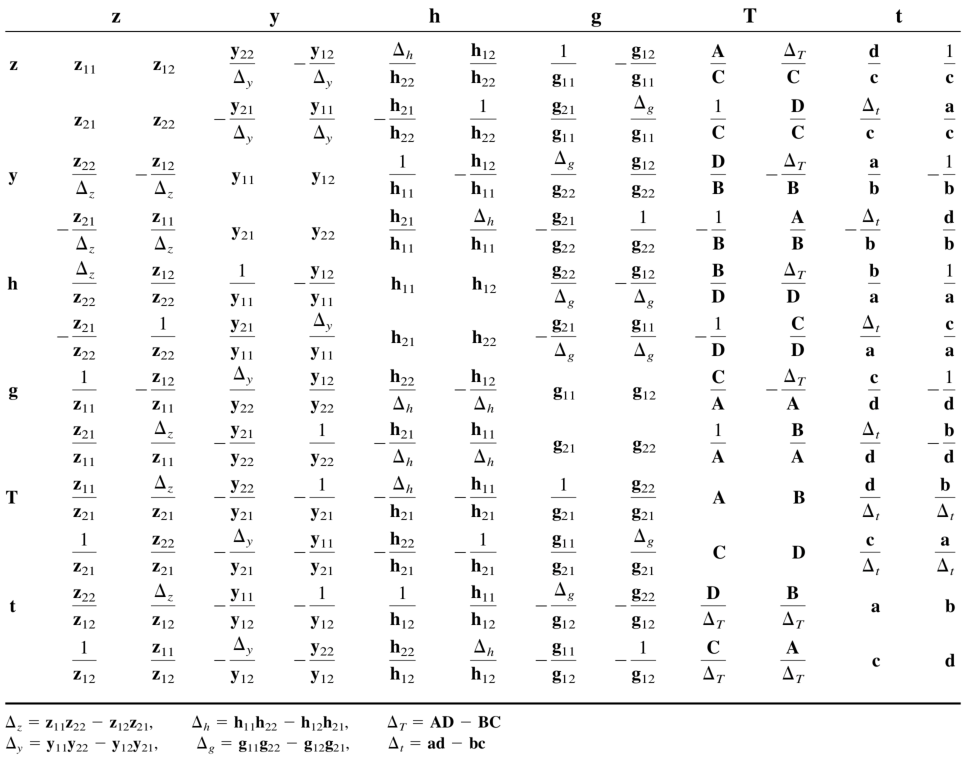
\includegraphics[height=4cm]{../figs/Tabla_Parametros.pdf}


\subsubsection{Reciprocidad}
\label{sec:org8de0a87}
A partir de las relaciones ya obtenidas para impedancia y admitancia, utilizando la tabla anterior obtenemos la relación para parámetros híbridos y de transmisión:
\[
\left.
\begin{array}{l}
  \mathbf{z_{12}} = \mathbf{z_{21}}\\
  \mathbf{y_{12}} = \mathbf{y_{21}}\\
\end{array}
\right\} \rightarrow
\left\{
\begin{array}{l}
  \mathbf{h_{12}} = - \mathbf{h_{21}}\\
  \mathbf{g_{12}} = - \mathbf{g_{21}}\\
  \mathbf{A} \mathbf{D} - \mathbf{B} \mathbf{C} = 1\\
  \mathbf{a} \mathbf{d} - \mathbf{b} \mathbf{c} = 1\\
\end{array}
\right.
\]


\subsubsection{Simetría}
\label{sec:org32ff848}
A partir de las relaciones ya obtenidas para impedancia y admitancia, utilizando la tabla anterior obtenemos la relación para parámetros híbridos y de transmisión:
\[
\left.
\begin{array}{l}
  \mathbf{z_{11}} = \mathbf{z_{22}}\\
  \mathbf{y_{11}} = \mathbf{y_{22}}\\
\end{array}
\right\} \rightarrow
\left\{
\begin{array}{l}
  \mathbf{h_{11}} \cdot \mathbf{h_{22}} - \mathbf{h_{12}}^2 = 1\\
  \mathbf{g_{11}} \cdot \mathbf{g_{22}} - \mathbf{g_{12}}^2 = 1\\
  \mathbf{A} =  \mathbf{D}\\
  \mathbf{a} =  \mathbf{d}\\
\end{array}
\right.
\]

Además:

\[
  \boxed{[\mathbf{T}] = [\mathbf{t}]}
\]


\section{Cuadripolos entre Dipolos Terminales}
\label{sec:org4eb70ca}

\subsection{Situación General}
\label{sec:orgf52f6e2}
\subsubsection{}
\label{sec:org495ece7}

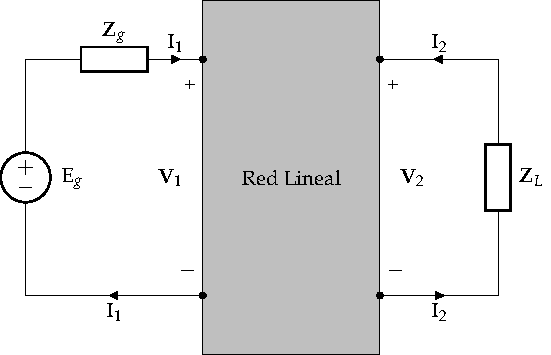
\includegraphics[height=4cm]{../figs/cuadripolo_cargado_fuente_tension.pdf}


\begin{align*}
  \mathbf{U}_1 &= \mathbf{E}_g - \mathbf{Z}_g \cdot \mathbf{I}_1\\
  \mathbf{U}_2 &= - \mathbf{Z}_L \cdot \mathbf{I}_2\\
\end{align*}

\subsubsection{}
\label{sec:orgc9420fa}

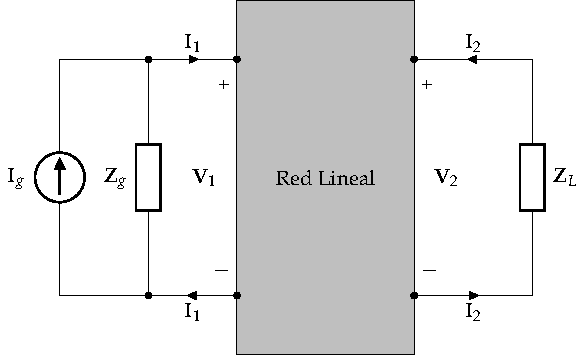
\includegraphics[height=4cm]{../figs/cuadripolo_cargado_fuente_corriente.pdf}


\begin{align*}
  \mathbf{U}_1 &= (\mathbf{I}_g - \mathbf{I}_1) \cdot \mathbf{Z}_g\\
  \mathbf{U}_2 &= - \mathbf{Z}_L \cdot \mathbf{I}_2\\
\end{align*}

\subsubsection{Ganancia}
\label{sec:orge1f4b88}

\begin{enumerate}
\item \hfill{}\textsc{BMCOL}
\label{sec:org1a393ee}

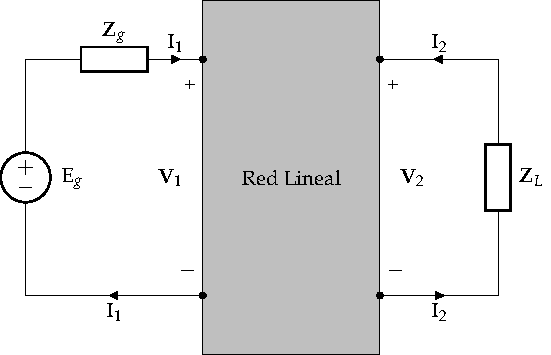
\includegraphics[height=4cm]{../figs/cuadripolo_cargado_fuente_tension.pdf}


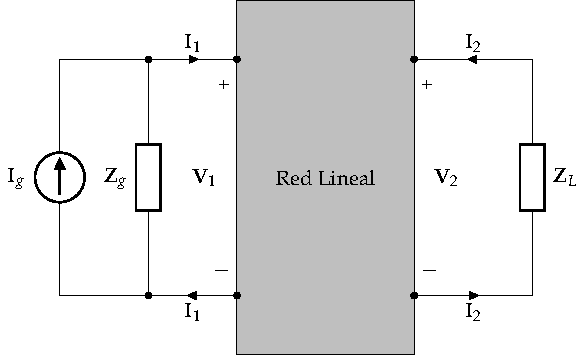
\includegraphics[height=4cm]{../figs/cuadripolo_cargado_fuente_corriente.pdf}



\item \hfill{}\textsc{BMCOL}
\label{sec:org77ac402}
\begin{itemize}
\item Ganancia de Tensión
\end{itemize}
\[
\mathbf{A}_V = \frac{\mathbf{U}_2}{\mathbf{E}_g}
\]
\begin{itemize}
\item Ganancia de Corriente
\end{itemize}
\[
\mathbf{A}_I = \frac{\mathbf{I}_2}{\mathbf{I}_g}
\]
\end{enumerate}

\subsubsection{Impedancia}
\label{sec:org591ea39}
\begin{enumerate}
\item \hfill{}\textsc{BMCOL}
\label{sec:orgd9d6752}

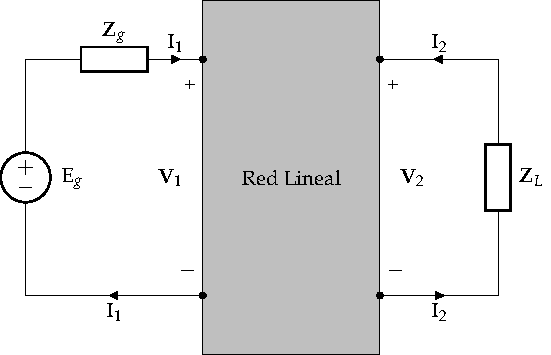
\includegraphics[height=4cm]{../figs/cuadripolo_cargado_fuente_tension.pdf}


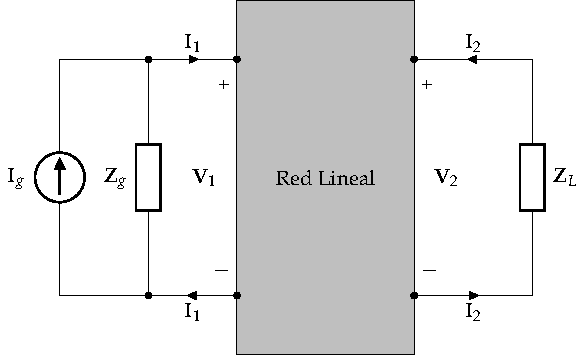
\includegraphics[height=4cm]{../figs/cuadripolo_cargado_fuente_corriente.pdf}



\item \hfill{}\textsc{BMCOL}
\label{sec:orgc27df88}
\begin{itemize}
\item Impedancia de Entrada
\end{itemize}
\[
\mathbf{Z}_i = \frac{\mathbf{U}_1}{\mathbf{I}_1}
\]

\begin{itemize}
\item Impedancia de Salida
\end{itemize}
\[
\mathbf{Z}_o = \left.\frac{\mathbf{U}_2}{\mathbf{I}_2}\right\rvert_{\mathbf{E}_g = 0}
\]
\end{enumerate}

\subsubsection{Transferencia}
\label{sec:orgb5d33e6}
\begin{enumerate}
\item \hfill{}\textsc{BMCOL}
\label{sec:org6258e98}

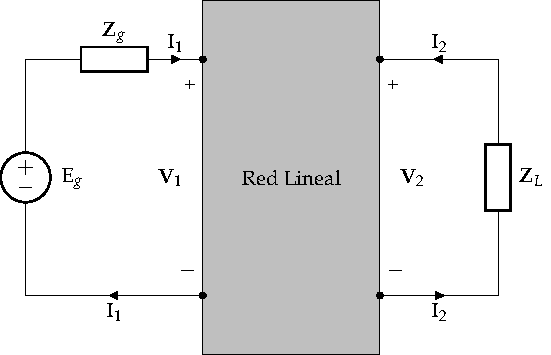
\includegraphics[height=4cm]{../figs/cuadripolo_cargado_fuente_tension.pdf}


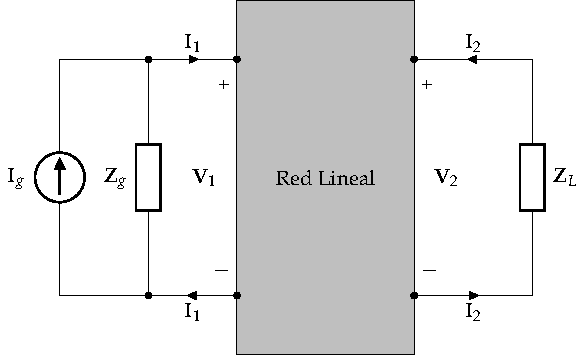
\includegraphics[height=4cm]{../figs/cuadripolo_cargado_fuente_corriente.pdf}



\item \hfill{}\textsc{BMCOL}
\label{sec:org8c9bbdc}
\begin{itemize}
\item Transadmitancia directa
\end{itemize}
\[
\mathbf{Y}_f = \frac{\mathbf{I}_2}{\mathbf{E}_g}
\]

\begin{itemize}
\item Transimpedancia directa
\end{itemize}
\[
\mathbf{Z}_f = \frac{\mathbf{U}_2}{\mathbf{I}_g}
\]
\end{enumerate}

\subsubsection{Ejercicio de Cálculo (1)}
\label{sec:orgce5d563}

Demuestra que la impedancia de entrada del circuito a la derecha de la fuente real expresada con parámetros de transmisión es:

\[
\mathbf{Z}_i = \frac{\mathbf{A} \mathbf{Z}_L + \mathbf{B}}{\mathbf{C}\mathbf{Z}_L + \mathbf{D}}
\]


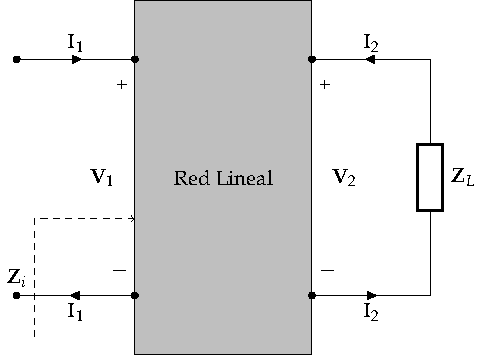
\includegraphics[height=4cm]{../figs/cuadripolo_cargado_impedancia_entrada.pdf}




\subsection{Impedancia de carga}

\begin{minipage}{0.5\textwidth}
  
    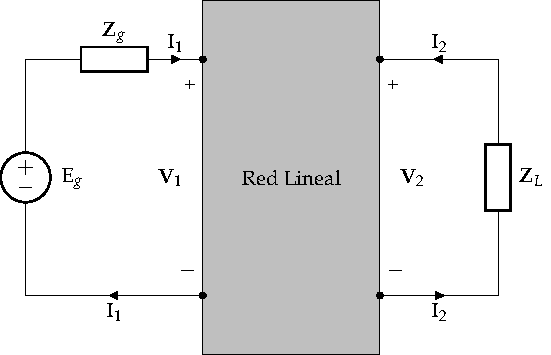
\includegraphics[height=4cm]{../figs/cuadripolo_cargado_fuente_tension.pdf}
  
\end{minipage}
\begin{minipage}{0.5\textwidth}
  \begin{align*}
    \mathbf{U}_1 &= \mathbf{E}_g - \mathbf{Z}_g \cdot \mathbf{I}_1\\
    \mathbf{U}_2 &= - \mathbf{Z}_L \cdot \mathbf{I}_2\\
  \end{align*}
\end{minipage}

\vspace{1cm}

Para obtener la máxima potencia en la salida del cuadripolo, la impedancia de carga $\mathbf{Z}_L$ deberá ser igual al conjugado de la impedancia de salida del cuadripolo, $\mathbf{Z}_L = \mathbf{Z}^*_o$, definida como:

\[
  \mathbf{Z}_o = \left.\dfrac{\mathbf{U}_2}{\mathbf{I}_2}\right\rvert_{\mathbf{E}_g = 0}
\]

Esta impedancia puede calcularse con cualquiera de las familias de parámetros anteriores. Por ejemplo, con los parámetros impedancia tendremos las siguientes ecuaciones:

\begin{align*}
  \mathbf{U}_1 &= - \mathbf{Z}_g \cdot \mathbf{I}_1\\
  \mathbf{U}_1 &= \mathbf{z}_{11} \mathbf{I}_1 + \mathbf{z}_{12} \mathbf{I}_2\\
  \mathbf{U}_2 &= \mathbf{z}_{21} \mathbf{I}_1 + \mathbf{z}_{22} \mathbf{I}_2\\
\end{align*}

Sustituyendo la primera ecuación en la segunda, y ésta a su vez en la tercera obtenemos:

\begin{equation*}
  \mathbf{Z}_o = \mathbf{z}_{22} - \dfrac{\mathbf{z}_{12} \cdot \mathbf{z}_{21}}{\mathbf{Z}_g + \mathbf{z}_{11}}
\end{equation*}

\subsection{Parámetros Imagen}
\label{sec:org5e458cf}

\subsubsection{Impedancia Característica}
\label{sec:orgcd34bb0}
Para un cuadripolo \textbf{recíproco} y \textbf{simétrico} se definen los parámetros imagen:

\begin{itemize}
\item \textbf{Impedancia característica}, \(\mathbf{Z}_o\): impedancia que, conectada en una puerta, hace que desde la otra puerta se vea la misma impedancia.
\end{itemize}
\[
  \mathbf{Z}_o = \frac{\mathbf{U}_1}{\mathbf{I}_1}
\]

\begin{enumerate}
\item \hfill{}\textsc{BMCOL}
\label{sec:org302b662}

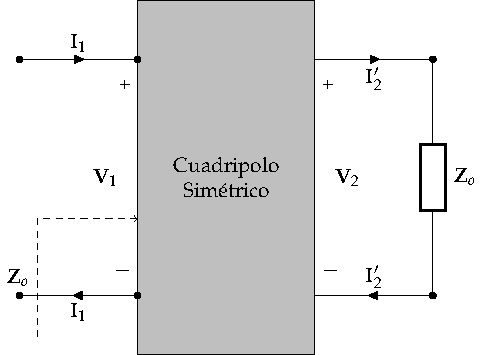
\includegraphics[height=4cm]{../figs/cuadripolo_impedancia_caracteristica.pdf}


\item \hfill{}\textsc{BMCOL}
\label{sec:orgc75359e}
\[
\mathbf{Z}_o = \frac{\mathbf{A} \mathbf{Z}_o + \mathbf{B}}{\mathbf{C}\mathbf{Z}_o + \mathbf{D}}
\]

\[
\mathbf{A} = \mathbf{D} \rightarrow \boxed{\mathbf{Z}_o = \pm \sqrt{\frac{\mathbf{B}}{\mathbf{C}}}}
\]
\end{enumerate}

\subsubsection{Impedancia Característica}
\label{sec:org7144bfc}

\begin{enumerate}
\item Atención
\label{sec:org9042c98}
La ecuación proporciona dos soluciones, una de las cuáles implicará una impedancia no viable (\emph{resistencia negativa}).
\[
\boxed{\mathbf{Z}_o = \pm \sqrt{\frac{\mathbf{B}}{\mathbf{C}}}}
\]
\end{enumerate}

\subsubsection{Función de Propagación}
\label{sec:orgf2ef1cc}
Para un cuadripolo \textbf{recíproco} y \textbf{simétrico} se definen los parámetros imagen:

\begin{itemize}
\item \textbf{Función de propagación}, \(\gamma\): relacionada con el cociente de potencias en las puertas del cuadripolo cuando una de ellas está cargada con \(\mathbf{Z}_o\)
\end{itemize}

\[
  \exp(2\gamma) = \frac{\mathbf{U}_1\mathbf{I}_1}{\mathbf{U}_2\mathbf{I}'_2}
\]

\begin{enumerate}
\item \hfill{}\textsc{BMCOL}
\label{sec:org884522a}

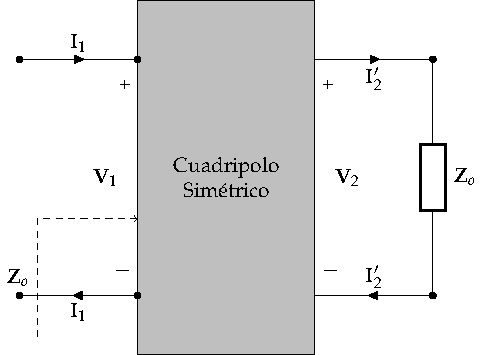
\includegraphics[height=4cm]{../figs/cuadripolo_impedancia_caracteristica.pdf}


\item \hfill{}\textsc{BMCOL}
\label{sec:org13d5d40}
\begin{align*}
  \mathbf{U}_1 &= \mathbf{I}_1 \mathbf{Z}_o\\
  \mathbf{U}_2 &= \mathbf{I}'_2 \mathbf{Z}_o
\end{align*}

\[
  \boxed{\exp(\gamma) = \frac{\mathbf{U}_1}{\mathbf{U}_2} = \frac{\mathbf{I}_1}{\mathbf{I}'_2}}
\]
\end{enumerate}


\subsubsection{Relación entre \(\mathbf{Z}_o\) y \(\gamma\)}
\label{sec:orgba47dd9}
\begin{enumerate}
\item \hfill{}\textsc{BMCOL}
\label{sec:org93db8e6}

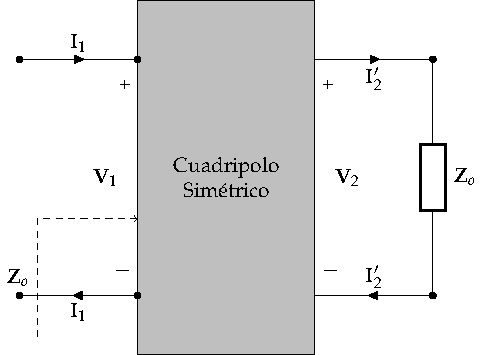
\includegraphics[height=4cm]{../figs/cuadripolo_impedancia_caracteristica.pdf}


\item \hfill{}\textsc{BMCOL}
\label{sec:org51048e6}
\begin{align*}
  \exp(\gamma) &= \frac{\mathbf{U}_1}{\mathbf{U}_2} =\\
               &= \frac{\mathbf{A}\mathbf{U}_2 + \mathbf{B}\mathbf{I}'_2}{\mathbf{U}_2} = \\
               &= \mathbf{A} + \mathbf{B}\frac{\mathbf{I}'_2}{\mathbf{U_2}}
\end{align*}

\[
  \boxed{\exp(\gamma) = \mathbf{A} + \frac{\mathbf{B}}{\mathbf{Z}_o}}
\]
\end{enumerate}

\subsubsection{Relación entre \(\mathbf{Z}_o\) y \(\gamma\)}
\label{sec:org2783cff}

Teniendo en cuenta la expresión de \(\mathbf{Z}_o\):
\[
  \left.
  \begin{array}{l}
    \mathbf{Z}_o = \pm \sqrt{\frac{\mathbf{B}}{\mathbf{C}}}\\
    \exp(\gamma) = \mathbf{A} + \frac{\mathbf{B}}{\mathbf{Z}_o}
  \end{array} \right\} \rightarrow
\boxed{\exp(\gamma) = \mathbf{A} \pm \sqrt{\mathbf{B}\mathbf{C}}}
\]

Además, teniendo en cuenta la relación de un cuadripolo recíproco y simétrico:

\[
  \mathbf{A}^2 - \mathbf{B}\mathbf{C} = 1 \rightarrow %
  \boxed{\exp(\gamma) = \mathbf{A} \pm \sqrt{\mathbf{A}^2 - 1}}
\]
\textbf{Atención} al signo que acompaña a las raíces cuadradas. Se debe elegir de forma que la parte real de \(\gamma\) sea acorde al cuadripolo.

\subsubsection{Transmisión a partir de Imagen}
\label{sec:org593cab5}

\[
\mathbf{A}^2 - \mathbf{B}\mathbf{C} = 1
\]

\begin{enumerate}
\item \hfill{}\textsc{BMCOL}
\label{sec:orgbfdda51}
\[
  e^\gamma = \mathbf{A} + \sqrt{\mathbf{A}^2 - 1}
\]

\[
  \mathbf{Z}_o = \sqrt{\frac{\mathbf{B}}{\mathbf{C}}}
\]

\item \hfill{}\textsc{BMCOL}
\label{sec:orgbb55298}
\begin{align*}
  \cosh(\gamma) &= \frac{e^\gamma + e^{-\gamma}}{2}\\
  \sinh(\gamma) &= \frac{e^\gamma - e^{-\gamma}}{2}\\
  \cosh^2(\gamma) &- \sinh^2(\gamma) = 1
\end{align*}

\item \hfill{}\textsc{B\_ignoreheading}
\label{sec:org51374bf}
\[
\boxed{
  \begin{array}{ll}
    \mathbf{A} = \cosh(\gamma) &
    \mathbf{B} = \mathbf{Z}_o \sinh(\gamma)\\
    \mathbf{C} = \sinh(\gamma)/\mathbf{Z}_o &
    \mathbf{D} = \cosh(\gamma)\\
  \end{array}
}
\]
\end{enumerate}

\subsubsection{Régimen Permanente Sinusoidal}
\label{sec:orgde43a7b}

Cuando el circuito funciona en régimen permanente sinusoidal:

\begin{itemize}
\item La función de propagación es un número complejo denominado constante de propagación.
\end{itemize}
\[
  \overline{\gamma} = \alpha + j\beta
\]
\begin{itemize}
\item Las tensiones y corrientes son fasores
\end{itemize}
\[
  \exp(\overline{\gamma}) = \exp(\alpha) \cdot \exp(j\beta) = \frac{\overline{U}_1}{\overline{U}_2} = \frac{\overline{I}_1}{\overline{I}'_2}
\]

\subsubsection{Régimen Permanente Sinusoidal}
\label{sec:org6afeb0f}
\begin{itemize}
\item \textbf{Constante de Atenuación} (cuando \(\alpha > 1\) el cuadripolo atenúa la salida respecto de la entrada)
\end{itemize}
\[
  \exp(\alpha) = \frac{U_1}{U_2} = \frac{I_1}{I_2}
\]
\begin{itemize}
\item \textbf{Constante de Fase} (desfase entre puertos)
\end{itemize}
\[
  \beta = \theta_{\overline{U}_1} - \theta_{\overline{U}_2} = \theta_{\overline{I}_1} - \theta_{\overline{I}'_2}
\]

\subsubsection{Atenuación de Potencia}
\label{sec:org3c1bb07}

\textbf{Cuando está conectada la impedancia característica}, las potencias activas en los puertos se expresan:

\begin{align*}
  P_1 &= U_1 I_1 \cos(\theta_o)\\
  P_2 &= U_2 I_2 \cos(\theta_o)
\end{align*}
donde \(\theta_o\) es el ángulo de la impedancia \(\overline{Z}_o\).

Por tanto, la relación de potencias activas es:

\[
\frac{P_1}{P_2} = \frac{U_1 I_1}{U_2 I_2}
\]
Teniendo en cuenta la expresión de la constante de atenuación, esta relación es:
\[
    \exp(\alpha) = \frac{U_1}{U_2} = \frac{I_1}{I_2} \rightarrow \boxed{\exp(2\alpha) = \frac{U_1 I_1}{U_2 I_1} = \frac{P_1}{P_2}}
\]

\section{Asociación de Cuadripolos}
\label{sec:org69d0c87}

\subsubsection{Conexiones}
\label{sec:orgf6e2051}

\begin{enumerate}
\item Definición
\label{sec:org531ded7}
\begin{itemize}
\item \textbf{Serie}: misma corriente, suma de tensiones
\item \textbf{Paralelo}: misma tensión, suma de corrientes
\end{itemize}
\item Catálogo
\label{sec:org94028dc}
\begin{itemize}
\item Serie-Serie: \textbf{parámetros impedancia}
\item Paralelo-Paralelo: \textbf{parámetros admitancia}
\item Serie-Paralelo: \textbf{parámetros híbridos}
\item Paralelo-Serie: \textbf{parámetros híbridos inversos}
\item Cascada: \textbf{parámetros transmisión/imagen}
\end{itemize}
\end{enumerate}
\subsection{Asociación Serie-Serie}
\label{sec:orgf8c64c4}

\subsubsection{Conexión}
\label{sec:org93220a5}

\begin{enumerate}
\item \hfill{}\textsc{BMCOL}
\label{sec:orgfbc403e}

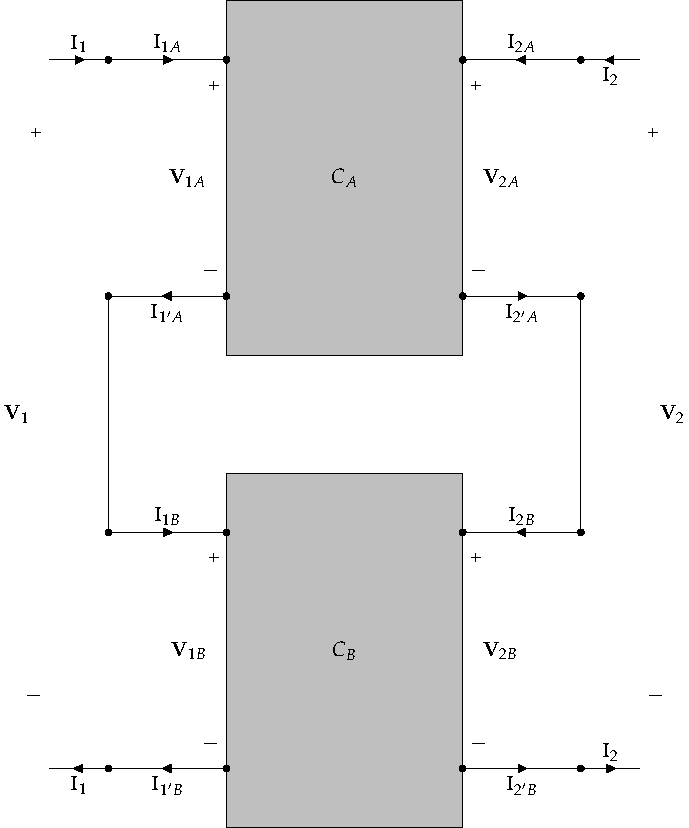
\includegraphics[height=4cm]{../figs/serie-serie.pdf}




\item \hfill{}\textsc{BMCOL}
\label{sec:orgb817874}
\begin{enumerate}
\item Tensiones
\label{sec:orgbdd8729}
\begin{align*}
  \mathbf{U}_1 &= \mathbf{U}_{1A} + \mathbf{U}_{1B}\\
  \mathbf{U}_2 &= \mathbf{U}_{2A} + \mathbf{U}_{2B}
\end{align*}

\item Condición de Puerto
\label{sec:org70529d0}
\begin{align*}
  \mathbf{I}_{1A} &= \mathbf{I}_{1'A}\\
  \mathbf{I}_{1B} &= \mathbf{I}_{1'B}\\
  \mathbf{I}_{2A} &= \mathbf{I}_{2'A}\\
  \mathbf{I}_{2B} &= \mathbf{I}_{2'B}
\end{align*}
\end{enumerate}
\end{enumerate}

\subsubsection{Cuadripolo Equivalente}
\label{sec:orga827299}
\begin{enumerate}
\item \hfill{}\textsc{BMCOL}
\label{sec:org213121f}

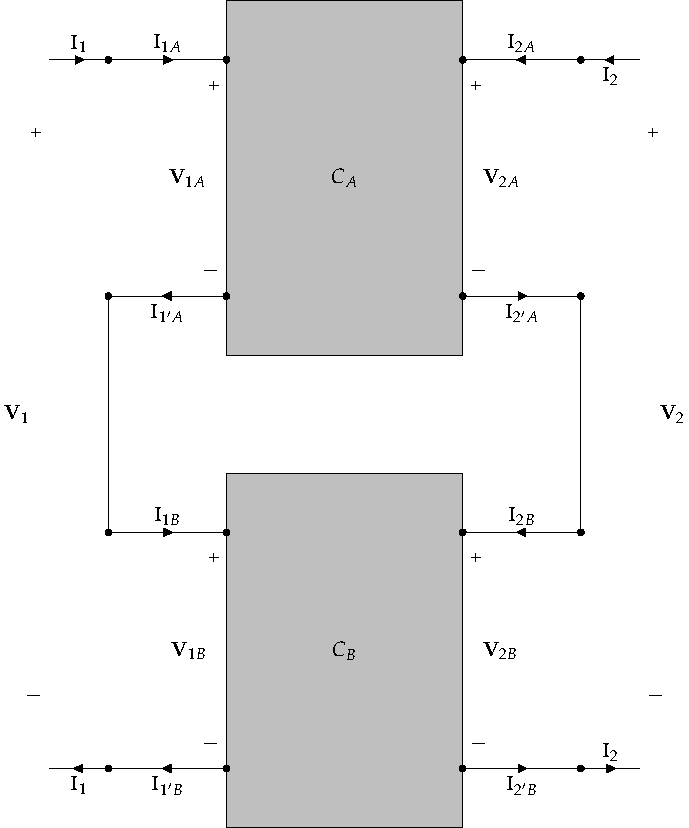
\includegraphics[height=4cm]{../figs/serie-serie.pdf}



\item \hfill{}\textsc{BMCOL}
\label{sec:org38dbe81}
\begin{enumerate}
\item Parámetros Impedancia
\label{sec:orgb198b8f}
\begin{align*}
  [\mathbf{U}_A] &= [\mathbf{Z}_A] \cdot [\mathbf{I}_A]\\
  [\mathbf{U}_B] &= [\mathbf{Z}_B] \cdot [\mathbf{I}_B]
\end{align*}

\item Cuadripolo Equivalente
\label{sec:org2696460}
\[
  \boxed{[\mathbf{Z}] = [\mathbf{Z}_A] + [\mathbf{Z}_B]}
\]
\end{enumerate}
\end{enumerate}

\subsubsection{Interacción}
\label{sec:org9daf72f}
\begin{enumerate}
\item \hfill{}\textsc{BMCOL}
\label{sec:orgfd071da}

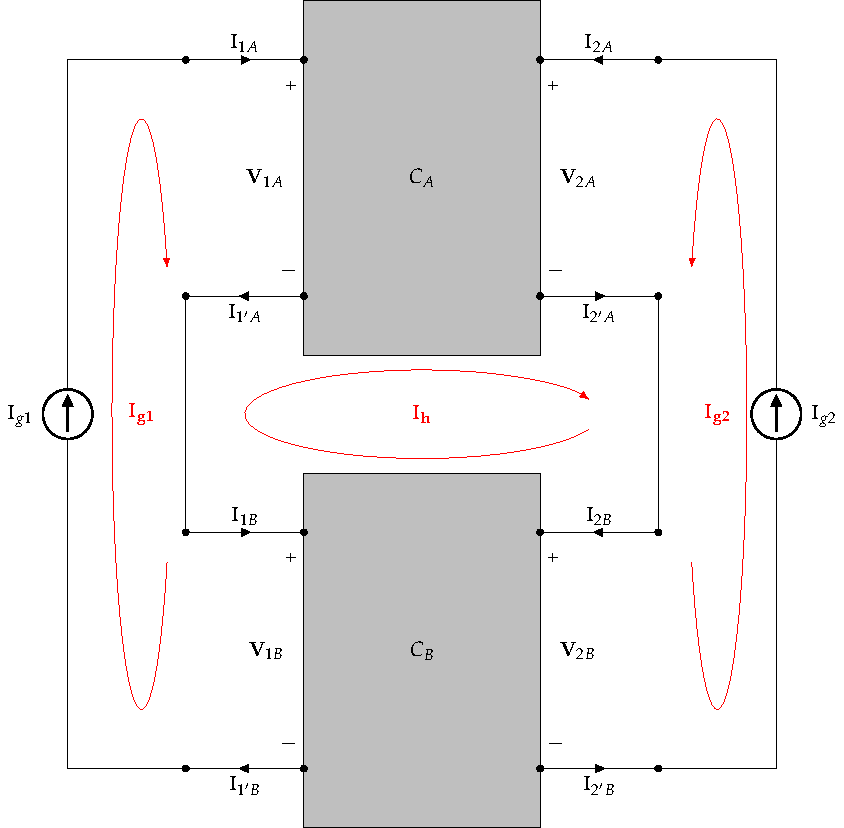
\includegraphics[height=5cm]{../figs/serie-serie-interaccion.pdf}

\item \hfill{}\textsc{BMCOL}
\label{sec:org009a6eb}
\begin{itemize}
\item Entrada
\end{itemize}
\begin{align*}
  \mathbf{I}_{1A} &= \mathbf{I}_{g1}\\
  \mathbf{I}_{1'A} &= \mathbf{I}_{g1} - \mathbf{I}_h
\end{align*}
\begin{itemize}
\item Salida
\end{itemize}
\begin{align*}
  \mathbf{I}_{2A} &= \mathbf{I}_{g2}\\
  \mathbf{I}_{2'A} &= \mathbf{I}_{g2}  + \mathbf{I}_h
\end{align*}
\begin{itemize}
\item Condición de Puerto
\end{itemize}
\[
\boxed{\mathbf{I}_h = 0}
\]
\end{enumerate}
\subsubsection{Interacción}
\label{sec:org45b1cf7}
Si no hay interacción, al aplicar superposición la corriente de circulación debe ser nula \textbf{en ambos casos}.
\begin{enumerate}
\item \hfill{}\textsc{BMCOL}
\label{sec:org7b3b505}

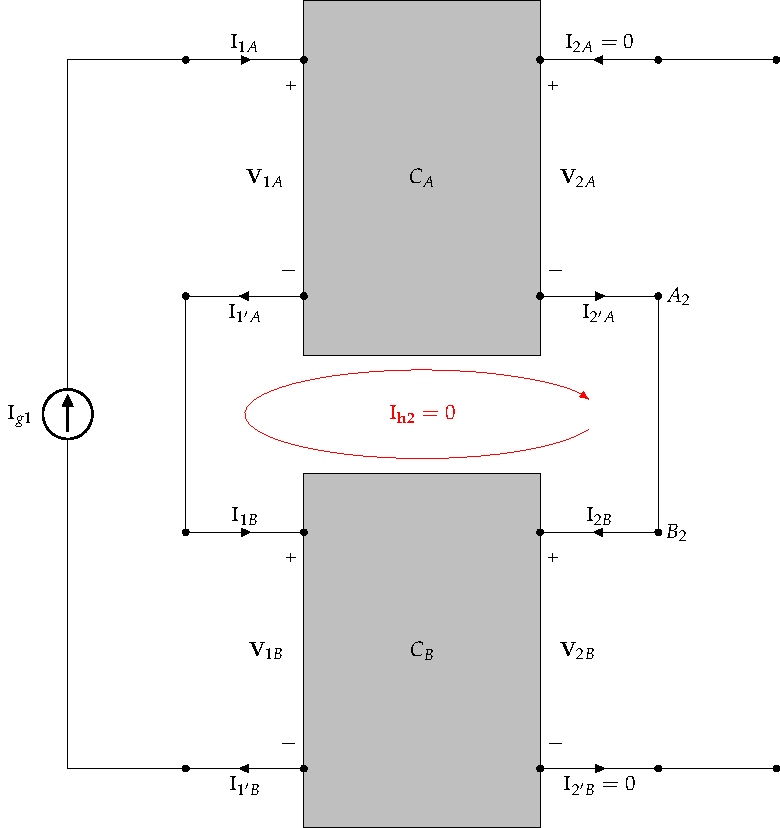
\includegraphics[height=5cm]{../figs/serie-serie-superposicion-entrada.pdf}

\item \hfill{}\textsc{BMCOL}
\label{sec:orgfc7026f}

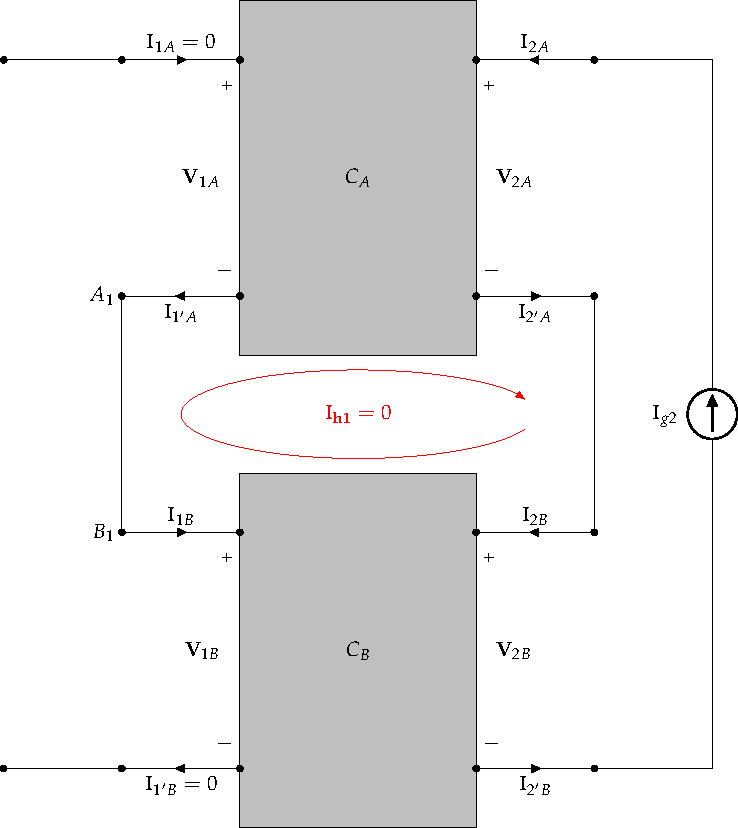
\includegraphics[height=5cm]{../figs/serie-serie-superposicion-salida.pdf}

\end{enumerate}

\subsubsection{Test de Brune}
\label{sec:org9a27190}
Aplicando superposición desconectamos los cuadripolos: \textbf{si no hay interacción, no habrá cambio de tensión}.
\begin{enumerate}
\item \hfill{}\textsc{BMCOL}
\label{sec:org3157d40}

\includegraphics[height=5cm]{../figs/serie-serie-brune-entrada.pdf}

\item \hfill{}\textsc{BMCOL}
\label{sec:org355faf6}

\includegraphics[height=5cm]{../figs/serie-serie-brune-salida.pdf}

\end{enumerate}


\subsubsection{Métodos para evitar interacción}
\label{sec:org033b270}

\includegraphics[height=4cm]{../figs/serie-serie-transformador.pdf}


\subsubsection{Métodos para evitar interacción}
\label{sec:org7265967}

\includegraphics[height=4cm]{../figs/serie-serie-corto.pdf}


\subsection{Asociación Paralelo-Paralelo}
\label{sec:org3afa958}
\subsubsection{Conexión}
\label{sec:org39169d7}
\begin{enumerate}
\item \hfill{}\textsc{BMCOL}
\label{sec:org8edd165}

\includegraphics[height=4cm]{../figs/paralelo-paralelo.pdf}

\item \hfill{}\textsc{BMCOL}
\label{sec:orgc8c6f3c}
\begin{enumerate}
\item Corrientes
\label{sec:orgb710c53}
\begin{align*}
  \mathbf{I}_1 &= \mathbf{I}_{1A} + \mathbf{I}_{1B}\\
  \mathbf{I}_2 &= \mathbf{I}_{2A} + \mathbf{I}_{2B}
\end{align*}

\item Condición de Puerto
\label{sec:orgf90580b}
\begin{align*}
  \mathbf{I}_{1A} &= \mathbf{I}_{1'A}\\
  \mathbf{I}_{1B} &= \mathbf{I}_{1'B}\\
  \mathbf{I}_{2A} &= \mathbf{I}_{2'A}\\
  \mathbf{I}_{2B} &= \mathbf{I}_{2'B}
\end{align*}
\end{enumerate}
\end{enumerate}

\subsubsection{Cuadripolo Equivalente}
\label{sec:org0bc310b}
\begin{enumerate}
\item \hfill{}\textsc{BMCOL}
\label{sec:org0d6fdf5}

\includegraphics[height=4cm]{../figs/paralelo-paralelo.pdf}



\item \hfill{}\textsc{BMCOL}
\label{sec:org582370f}
\begin{enumerate}
\item Parámetros Admitancia
\label{sec:org0aeffe8}
\begin{align*}
  [\mathbf{I}_A] &= [\mathbf{Y}_A] \cdot [\mathbf{U}_A]\\
  [\mathbf{I}_B] &= [\mathbf{Y}_B] \cdot [\mathbf{U}_B]
\end{align*}

\item Cuadripolo Equivalente
\label{sec:orgdcc9958}
\[
  \boxed{[\mathbf{Y}] = [\mathbf{Y}_A] + [\mathbf{Y}_B]}
\]
\end{enumerate}
\end{enumerate}
\subsubsection{Interacción}
\label{sec:orgd584cd4}

\includegraphics[height=4cm]{../figs/paralelo-paralelo-interaccion.pdf}

\subsubsection{Interacción}
\label{sec:orgf1d8a5b}
Si no hay interacción, al aplicar superposición la corriente de circulación debe ser nula \textbf{en ambos casos}.
\begin{enumerate}
\item \hfill{}\textsc{BMCOL}
\label{sec:orgaa86e5c}

\includegraphics[height=5cm]{../figs/paralelo-paralelo-superposicion-entrada.pdf}

\item \hfill{}\textsc{BMCOL}
\label{sec:org5b95701}

\includegraphics[height=5cm]{../figs/paralelo-paralelo-superposicion-salida.pdf}

\end{enumerate}

\subsubsection{Test de Brune}
\label{sec:org2591d22}
Aplicando superposición desconectamos los cuadripolos: \textbf{si no hay interacción, no habrá cambio de tensión}.
\begin{enumerate}
\item \hfill{}\textsc{BMCOL}
\label{sec:org951e127}

\includegraphics[height=5cm]{../figs/paralelo-paralelo-brune-entrada.pdf}

\item \hfill{}\textsc{BMCOL}
\label{sec:orgc2f98c6}

\includegraphics[height=5cm]{../figs/paralelo-paralelo-brune-salida.pdf}

\end{enumerate}

\subsubsection{Test de Brune}
\label{sec:org199da56}
Aplicando superposición desconectamos los cuadripolos: \textbf{si no hay interacción, no habrá cambio de tensión}.
\begin{enumerate}
\item \hfill{}\textsc{BMCOL}
\label{sec:orge3bd0e3}

\includegraphics[height=5cm]{../figs/paralelo-paralelo-brune-entrada2.pdf}

\item \hfill{}\textsc{BMCOL}
\label{sec:org745f22c}

\includegraphics[height=5cm]{../figs/paralelo-paralelo-brune-salida2.pdf}

\end{enumerate}

\subsubsection{Métodos para evitar interacción}
\label{sec:org31cbc7e}

\includegraphics[height=4cm]{../figs/paralelo-paralelo-transformador.pdf}

\subsubsection{Métodos para evitar interacción}
\label{sec:org3abee48}

\includegraphics[height=4cm]{../figs/paralelo-paralelo-corto.pdf}

\subsection{Asociación Serie-Paralelo}
\label{sec:orgc44bd68}
\subsubsection{Conexión}
\label{sec:orgcba0d44}
\begin{enumerate}
\item \hfill{}\textsc{BMCOL}
\label{sec:orgb6b388b}

\includegraphics[height=4cm]{../figs/serie-paralelo.pdf}

\item \hfill{}\textsc{BMCOL}
\label{sec:org547d1ed}
\begin{enumerate}
\item Relaciones
\label{sec:org9cf9c76}
\begin{align*}
  \mathbf{U}_1 &= \mathbf{U}_{1A} + \mathbf{U}_{1B}\\
  \mathbf{I}_2 &= \mathbf{I}_{2A} + \mathbf{I}_{2B}
\end{align*}

\item Cuadripolo Equivalente
\label{sec:orgb751890}
\[
  \boxed{[\mathbf{H}] = [\mathbf{H}_A] + [\mathbf{H}_B]}
\]
\end{enumerate}
\end{enumerate}
\subsubsection{Test de Brune}
\label{sec:orgb1acd8e}
Aplicando superposición desconectamos los cuadripolos: \textbf{si no hay interacción, no habrá cambio de tensión}.
\begin{enumerate}
\item \hfill{}\textsc{BMCOL}
\label{sec:orge70fe59}

\includegraphics[height=5cm]{../figs/serie-paralelo-brune-entrada.pdf}

\item \hfill{}\textsc{BMCOL}
\label{sec:orgfd2f144}

\includegraphics[height=5cm]{../figs/serie-paralelo-brune-salida.pdf}

\end{enumerate}

\subsection{Asociación Paralelo-Serie}
\label{sec:orgd91e058}
\subsubsection{Conexión}
\label{sec:org5e14c91}
\begin{enumerate}
\item \hfill{}\textsc{BMCOL}
\label{sec:org43cb61d}

\includegraphics[height=4cm]{../figs/paralelo-serie.pdf}

\item \hfill{}\textsc{BMCOL}
\label{sec:orge5d2f92}
\begin{enumerate}
\item Relaciones
\label{sec:orge6945d2}
\begin{align*}
  \mathbf{I}_1 &= \mathbf{I}_{1A} + \mathbf{I}_{1B}\\
  \mathbf{U}_2 &= \mathbf{U}_{2A} + \mathbf{U}_{2B}
\end{align*}

\item Cuadripolo Equivalente
\label{sec:orgd5cfc0b}
\[
  \boxed{[\mathbf{G}] = [\mathbf{G}_A] + [\mathbf{G}_B]}
\]
\end{enumerate}
\end{enumerate}

\subsubsection{Test de Brune}
\label{sec:org7667a46}
Aplicando superposición desconectamos los cuadripolos: \textbf{si no hay interacción, no habrá cambio de tensión}.
\begin{enumerate}
\item \hfill{}\textsc{BMCOL}
\label{sec:orga5560fd}

\includegraphics[height=5cm]{../figs/paralelo-serie-brune-entrada.pdf}

\item \hfill{}\textsc{BMCOL}
\label{sec:org4d90737}

\includegraphics[height=5cm]{../figs/paralelo-serie-brune-salida.pdf}

\end{enumerate}
\subsection{Asociación Cascada}
\label{sec:org0d5b08b}

\subsubsection{Conexión}
\label{sec:org41e64cd}

\includegraphics[height=4cm]{../figs/cascada.pdf}


\begin{align*}
  \mathbf{U}_{2A} &= \mathbf{U}_{1B}\\
  \mathbf{I}'_{2A} &= \mathbf{I}_{1B}
\end{align*}


\[
  \boxed{[\mathbf{T}] = [\mathbf{T}_A] \cdot [\mathbf{T}_B]}
\]

%%% Local Variables:
%%% mode: latex
%%% TeX-master: "TC"
%%% ispell-local-dictionary: "castellano"
%%% End:
